\documentclass[review]{elsarticle}
%DIF LATEXDIFF DIFFERENCE FILE
%DIF DEL HFNG NIM_V2.tex             Wed Dec 20 08:49:29 2017
%DIF ADD HFNG NIM_Voyles_edits.tex   Sat Dec 23 20:31:30 2017

\usepackage{lineno,hyperref}
%DIF 4a4
\usepackage[utf8]{inputenc} %DIF > 
%DIF -------

%DIF 5a6
 %DIF > 
%DIF -------
\usepackage{graphicx}
\usepackage{float}
\usepackage{amsmath}
%DIF 8a10-11
\usepackage{amssymb} %DIF > 
 %DIF > 
%DIF -------
\usepackage{gensymb}
%DIF 9a13
\usepackage{siunitx} %DIF > 
%DIF -------
\usepackage[caption=false]{subfig}
%DIF 10a15-55
\usepackage[colorinlistoftodos]{todonotes} %DIF > 
\usepackage [autostyle, english = american]{csquotes} %DIF > 
 %DIF > 
\usepackage{amsmath} %DIF > 
\usepackage[version=3]{mhchem}  %DIF > 
% \usepackage{fixltx2e} %DIF > 
% \usepackage{refcount} %DIF > 
% \usepackage{siunitx} %DIF > 
% \usepackage{lastpage} %DIF > 
% \usepackage{textcomp} %DIF > 
\usepackage{mathtools} %DIF > 
 %DIF > 
\usepackage{xfrac} %DIF > 
% \usepackage{lmodern} %DIF > 
% \usepackage{cool} %DIF > 
% \usepackage{cancel} %DIF > 
\usepackage{microtype} %DIF > 
\usepackage{listings} %DIF > 
\usepackage{mcode} %DIF > 
% \usepackage{longtable} %DIF > 
% \usepackage{subcaption} %DIF > 
% \usepackage{booktabs,siunitx} %DIF > 
\usepackage{gensymb} %DIF > 
% \usepackage[normalem]{ulem} %DIF > 
 %DIF > 
% \usepackage{mathtools, cuted} %DIF > 
 %DIF > 
 %DIF > 
% \usepackage[usenames,dvipsnames,svgnames,table]{xcolor} %DIF > 
\usepackage{color} %DIF > 
 %DIF > 
% \usepackage[colorinlistoftodos]{todonotes} %DIF > 
 %DIF > 
% \usepackage[section]{placeins} %DIF > 
% \usepackage{multirow} %DIF > 
 %DIF > 
% \usepackage{lineno} %DIF > 
 %DIF > 
 %DIF > 
 %DIF > 
 %DIF > 
%DIF -------
\captionsetup{font=normalsize,labelfont={bf,sf}}
%DIF 11a57-59
 %DIF > 
\newcommand{\comment}[1]{\todo[color=blue!20!white,inline]{ASV: #1}}  %DIF > 
 %DIF > 
%DIF -------

\modulolinenumbers[1]

\journal{Journal of Nuclear Instruments and Methods}

%%%%%%%%%%%%%%%%%%%%%%%
%% Elsevier bibliography styles
%%%%%%%%%%%%%%%%%%%%%%%
%% To change the style, put a % in front of the second line of the current style and
%% remove the % from the second line of the style you would like to use.
%%%%%%%%%%%%%%%%%%%%%%%

%% Numbered
%\bibliographystyle{model1-num-names}

%% Numbered without titles
%\bibliographystyle{model1a-num-names}

%% Harvard
%\bibliographystyle{model2-names.bst}\biboptions{authoryear}

%% Vancouver numbered
%\usepackage{numcompress}\bibliographystyle{model3-num-names}

%% Vancouver name/year
%\usepackage{numcompress}\bibliographystyle{model4-names}\biboptions{authoryear}

%% APA style
%\bibliographystyle{model5-names}\biboptions{authoryear}

%% AMA style
%\usepackage{numcompress}\bibliographystyle{model6-num-names}

%% `Elsevier LaTeX' style
\bibliographystyle{elsarticle-num}
%%%%%%%%%%%%%%%%%%%%%%%
%DIF PREAMBLE EXTENSION ADDED BY LATEXDIFF
%DIF UNDERLINE PREAMBLE %DIF PREAMBLE
\RequirePackage[normalem]{ulem} %DIF PREAMBLE
\RequirePackage{color}\definecolor{RED}{rgb}{1,0,0}\definecolor{BLUE}{rgb}{0,0,1} %DIF PREAMBLE
\providecommand{\DIFadd}[1]{{\protect\color{blue}\uwave{#1}}} %DIF PREAMBLE
\providecommand{\DIFdel}[1]{{\protect\color{red}\sout{#1}}}                      %DIF PREAMBLE
%DIF SAFE PREAMBLE %DIF PREAMBLE
\providecommand{\DIFaddbegin}{} %DIF PREAMBLE
\providecommand{\DIFaddend}{} %DIF PREAMBLE
\providecommand{\DIFdelbegin}{} %DIF PREAMBLE
\providecommand{\DIFdelend}{} %DIF PREAMBLE
%DIF FLOATSAFE PREAMBLE %DIF PREAMBLE
\providecommand{\DIFaddFL}[1]{\DIFadd{#1}} %DIF PREAMBLE
\providecommand{\DIFdelFL}[1]{\DIFdel{#1}} %DIF PREAMBLE
\providecommand{\DIFaddbeginFL}{} %DIF PREAMBLE
\providecommand{\DIFaddendFL}{} %DIF PREAMBLE
\providecommand{\DIFdelbeginFL}{} %DIF PREAMBLE
\providecommand{\DIFdelendFL}{} %DIF PREAMBLE
%DIF END PREAMBLE EXTENSION ADDED BY LATEXDIFF

\begin{document}
	
	\begin{frontmatter}

	\title{Design, \DIFdelbegin \DIFdel{Construction}\DIFdelend \DIFaddbegin \DIFadd{construction}\DIFaddend , and \DIFdelbegin \DIFdel{Characterization }\DIFdelend \DIFaddbegin \DIFadd{characterization }\DIFaddend of a \DIFdelbegin \DIFdel{Compact }\DIFdelend \DIFaddbegin \DIFadd{compact }\DIFaddend DD \DIFdelbegin \DIFdel{Neutron Generator Designed }\DIFdelend \DIFaddbegin \DIFadd{neutron generator designed }\DIFaddend for $^{40}Ar/^{39}Ar$ \DIFdelbegin \DIFdel{Geochronology}\DIFdelend \DIFaddbegin \DIFadd{geochronology}\DIFaddend }
	%\tnotetext[mytitlenote]{Fully documented templates are available in the elsarticle package on \href{http://www.ctan.org/tex-archive/macros/latex/contrib/elsarticle}{CTAN}.}
	\iffalse
	%% Group authors per affiliation:
	\author[UCB]{Mauricio Ayllon\corref{mycorrespondingauthor}}
	\ead{mayllon@berkeley.edu}
	\author[UCB]{Cory Waltz}
		\author[livermore]{Joseph Bauer}
	\author[geochronology]{Tim Becker}
	\author[UCB]{Lee Bernstein}
	\author[UCB]{Ka-Ngo Leung}
	\author[UCB]{Leo Kirsch}
	\author[geochronology]{Paul Renne}
	\author[UCB]{Karl Van Bibber}

	\cortext[mycorrespondingauthor]{Corresponding author}

	\address[UCB]{Department of Nuclear Engineering, University of California, Berkeley, CA 94720, USA}
	\address[livermore]{Lawrence Livermore National Laboratory, Livermore, CA 94550, USA}
	\address[geochronology]{Berkeley Geochronology Center, 2455 Ridge Road,Berkeley, CA 94720, USA}

	\fi

\begin{abstract}

A  \DIFdelbegin \DIFdel{facility based on a }\DIFdelend next-generation, high-flux\DIFaddbegin \DIFadd{, compact }\DIFaddend DD neutron generator has been designed, \DIFdelbegin \DIFdel{constructed, }\DIFdelend commissioned, and characterized, and is now operational \DIFaddbegin \DIFadd{in a new facility  }\DIFaddend at the University of California\DIFaddbegin \DIFadd{, }\DIFaddend Berkeley. The generator\DIFdelbegin \DIFdel{is }\DIFdelend \DIFaddbegin \DIFadd{, originally }\DIFaddend designed for $^{40}Ar/^{39}Ar$ dating of geological materials\DIFdelbegin \DIFdel{. However, it has served numerous other applicationssuch as }\DIFdelend \DIFaddbegin \DIFadd{, has since served numerous additional applications, including }\DIFaddend medical isotope production studies, \DIFdelbegin \DIFdel{and others  are being planned }\DIFdelend \DIFaddbegin \DIFadd{with others  planned for the near future}\DIFaddend . In this work, we present \DIFdelbegin \DIFdel{a description }\DIFdelend \DIFaddbegin \DIFadd{an overview }\DIFaddend of the High Flux Neutron Generator (HFNG) \DIFdelbegin \DIFdel{that }\DIFdelend \DIFaddbegin \DIFadd{which }\DIFaddend includes simulation tools, analytical treatments, and experimental validation of results. The \DIFdelbegin \DIFdel{current yield is around $10^9\ n/s$ }\DIFdelend \DIFaddbegin \DIFadd{generator's current neutron yield is approximately $10^9$ n/s, }\DIFaddend with future development aimed at achieving an output of \DIFdelbegin \DIFdel{over $10^{10}\ n/s$}\DIFdelend \DIFaddbegin \DIFadd{more than $10^{10}$ n/s}\DIFaddend . Extensive analysis was performed in order to characterize the neutron yield, flux, and energy distribution at specific locations where samples \DIFdelbegin \DIFdel{can be irradiated. A particular }\DIFdelend \DIFaddbegin \DIFadd{may be loaded for irradiation. A notable }\DIFaddend design feature of the HFNG is \DIFdelbegin \DIFdel{irradiation of samples }\DIFdelend \DIFaddbegin \DIFadd{the possibility for  sample  irradiation }\DIFaddend internal to the cathode, just a few millimeters away from the neutron production site, thus maximizing the flux, while minimizing the total neutron fluence. Moreover, the deuterium ion beam optics \DIFdelbegin \DIFdel{was simulated and optimized with different extraction configurations}\DIFdelend \DIFaddbegin \DIFadd{were  and optimized by simulation for various extraction configurations, }\DIFaddend so as to provide a uniform neutron flux distribution and an acceptable heat load. Finally, experiments were performed in order to \DIFdelbegin \DIFdel{validate the aforementioned analysis}\DIFdelend \DIFaddbegin \DIFadd{benchmark the modeling and characterization of HFNG operation}\DIFaddend .   

\DIFaddbegin \comment{Paper's title capitalization changed to reflect NIM standards.}

\comment{Unsure what you mean by \enquote{simulation tools}  (\enquote{...which includes simulation tools, analytical treatments... }).  Please clarify.}

\comment{Define ``a few'' mm - it should be something like 8mm, if I recall.}

\DIFaddend \end{abstract}

	\begin{keyword}
		DD Neutron generator\sep MCNP simulations \sep ion beam optics \sep flux quantification \sep geochronology \sep activation foils \sep COMSOL Multiphysics
	\end{keyword}

\end{frontmatter}

	\linenumbers

\section{Introduction}


Fusion-based neutron generators are used in many fields of research, education, and industry. As opposed to \DIFaddbegin \DIFadd{many }\DIFaddend other neutron sources\DIFdelbegin \DIFdel{such as research }\DIFdelend \DIFaddbegin \DIFadd{, such as thermal }\DIFaddend reactors, neutron generators provide nearly monoenergetic neutrons, pose a lower proliferation \DIFdelbegin \DIFdel{and radiological }\DIFdelend risk, do not produce \DIFdelbegin \DIFdel{high level }\DIFdelend \DIFaddbegin \DIFadd{high-level }\DIFaddend waste, and can be made compact and portable\DIFdelbegin \DIFdel{, among other benefits}\DIFdelend . The most common reactions for \DIFdelbegin \DIFdel{this kind of generators }\DIFdelend \DIFaddbegin \DIFadd{such a generator }\DIFaddend are shown in Equations \ref{eq:reactionDD} \DIFdelbegin \DIFdel{and \ref{eq:reactionDT}}\DIFdelend \DIFaddbegin \DIFadd{(}\enquote{DD}\DIFadd{) and \ref{eq:reactionDT} (}\enquote{DT}\DIFadd{)}\DIFaddend . At low energies, DT reactions benefit from a resonance near 100 keV, which allows for a higher neutron yield at a given beam current. Around this energy, the \DIFaddbegin \DIFadd{neutron }\DIFaddend yield from a DT source is \DIFdelbegin \DIFdel{slightly more than two orders of magnitude higher }\DIFdelend \DIFaddbegin \DIFadd{approximately  a factor of 80  greater }\DIFaddend than that of a DD source. \DIFaddbegin \comment{This figure needs a citation, search in EXFOR/elsewhere.} \DIFaddend However, the \DIFdelbegin \DIFdel{neutron energy }\DIFdelend \DIFaddbegin \DIFadd{DT neutron energy spectrum }\DIFaddend is also much higher, which can be a significant disadvantage \DIFaddbegin \comment{How?  Give an example or two.}\DIFaddend , or even inapplicable for some purposes \DIFaddbegin \comment{Again, be specific.  Give an example.}\DIFaddend . Moreover, tritium poses greater radiological handling and licensing challenges. 

\begin{align} \label{eq:reactionDD}
&^{2}H +\DIFaddbegin \ \DIFaddend ^{2}H \rightarrow\DIFaddbegin \ \DIFaddend ^{3}He + n + 3.27\ MeV\ (50\%) \\
&^{2}H +\DIFaddbegin \ \DIFaddend ^{3}H \rightarrow\DIFaddbegin \ \DIFaddend ^{4}He + n + 17.6\ MeV \label{eq:reactionDT}
\end{align}


Neutron generators are \DIFdelbegin \DIFdel{being }\DIFdelend \DIFaddbegin \DIFadd{commonly }\DIFaddend used for a variety of applications including activation analysis, \DIFdelbegin \DIFdel{production of radioisotopes}\DIFdelend \DIFaddbegin \DIFadd{radioisotope production}\DIFaddend , fast neutron imaging, oil well logging, fundamental nuclear research, \DIFaddbegin \DIFadd{and }\DIFaddend nuclear data measurements \DIFdelbegin \DIFdel{, etc}\DIFdelend \DIFaddbegin \comment{You should probably cite a source or two to back up this claim}\DIFaddend . The High Flux Neutron Generator (HFNG)\DIFaddbegin \DIFadd{, }\DIFaddend located at the University of California, Berkeley\DIFaddbegin \DIFadd{, }\DIFaddend was designed and built by the \DIFdelbegin \DIFdel{Nuclear Engineering Department }\DIFdelend \DIFaddbegin \DIFadd{Department of Nuclear Engineering  }\DIFaddend and the Berkeley Geochronology Center (BGC)\DIFdelbegin \DIFdel{with a primary application being }\DIFdelend \DIFaddbegin \DIFadd{, with  primary application in }\DIFaddend the improvement of the \DIFdelbegin \DIFdel{$^{40}Ar/^{39}Ar$ }\DIFdelend \DIFaddbegin \DIFadd{$^{40}$Ar/$^{39}$Ar }\DIFaddend dating technique, which consists \DIFdelbegin \DIFdel{on }\DIFdelend \DIFaddbegin \DIFadd{of }\DIFaddend irradiating geological samples in order to produce measurable quantities of \DIFdelbegin \DIFdel{$^{39}Ar$ through the  reaction $^{39}K(n,p)^{39}Ar$}\DIFdelend \DIFaddbegin \DIFadd{$^{39}$Ar through the  $^{39}$K(n,p)$^{39}$Ar reaction}\DIFaddend . Currently, \DIFdelbegin \DIFdel{samples are sent to }\DIFdelend \DIFaddbegin \DIFadd{these samples must be  sent away to thermal }\DIFaddend reactors for neutron irradiation. A local source of DD neutrons would have many advantages in addition to convenience; the \DIFdelbegin \DIFdel{lower energy monochromatic }\DIFdelend \DIFaddbegin \DIFadd{lower-energy quasi-monoenergetic }\DIFaddend DD neutrons would result in more precise age determinations by eliminating argon recoil out of the samples, \DIFdelbegin \DIFdel{and }\DIFdelend \DIFaddbegin \DIFadd{in addition to reduced }\DIFaddend production of confounding isotopes \DIFdelbegin \DIFdel{that accompany }\DIFdelend \DIFaddbegin \DIFadd{which accompany irradiation via }\DIFaddend the use of \DIFdelbegin \DIFdel{higher energy }\DIFdelend \DIFaddbegin \DIFadd{higher-energy }\DIFaddend fission neutrons \cite{geochron}.

\DIFaddbegin \comment{I'd check on this claim of reduced contaminant isotopes relative to fission neutrons.  DD will give roughly 2.2-2.8 MeV neutrons, whereas only about 15\% of watt spectrum neutrons are born above 3 MeV.  I don't think its the high-energy fission neutrons which are the problem, but the massive amount of thermals, which will produce a ton of unwanted (n,$\gamma$) activities.  Check this either way.}

\DIFaddend Since its commissioning, the HFNG has been proven useful for a variety of \DIFdelbegin \DIFdel{other }\DIFdelend \DIFaddbegin \DIFadd{additional }\DIFaddend applications including Prompt Gamma Neutron Activation Analysis (PGNAA) for on-site gamma detector calibration, cross-section measurements \DIFdelbegin \DIFdel{of relevant radioisotopes in medicine \mbox{%DIFAUXCMD
\cite{np_paper}
}%DIFAUXCMD
, }\DIFdelend \DIFaddbegin \DIFadd{for emerging medical radioisotopes \mbox{%DIFAUXCMD
\cite{np_paper}
}%DIFAUXCMD
}\comment{Cite the n,p paper here, and make sure to update the paper's metadata: (\url{http://linkinghub.elsevier.com/retrieve/pii/S0168583X17308145})}\DIFadd{, the }\DIFaddend study of delayed \DIFdelbegin \DIFdel{gamma rays from fission of $^{238}U$, single event upset }\DIFdelend \DIFaddbegin \DIFadd{fission gamma rays in  $^{238}$U, inducing single event upsets }\DIFaddend (SEU) \DIFdelbegin \DIFdel{of CPUs to develop }\DIFdelend \DIFaddbegin \DIFadd{in CPUs for development of }\DIFaddend radiation hardened electronics, \DIFdelbegin \DIFdel{study of the behavior of  NaI detectors in a neutron field, and}\DIFdelend \DIFaddbegin \DIFadd{the study of  NaI detector response in neutron fields, and, }\DIFaddend most recently, cross-section measurements of \DIFdelbegin \DIFdel{$^{35}Cl(n,p)^{35}S$ and $^{35}Cl(n,\alpha)^{32}P$}\DIFdelend \DIFaddbegin \DIFadd{$^{35}$Cl(n,p)$^{35}$S and $^{35}$Cl(n,$\alpha)^{32}$P}\DIFaddend , which are of significant interest for the design of molten salt reactors. \DIFaddbegin \comment{I'd check with the people involved in each of these projects, to see if they have any citeable works for here.  In particular, I'm pretty sure Batch has a conference proceeding / publication for the Cl cross section work, and Leo has talked about the U238 fission gammas.}
\DIFaddend 

The HFNG \DIFdelbegin \DIFdel{works }\DIFdelend \DIFaddbegin \DIFadd{operates }\DIFaddend by accelerating positive deuterium ions towards a titanium target electrode biased \DIFdelbegin \DIFdel{up to }\DIFdelend \DIFaddbegin \DIFadd{at a }\DIFaddend -120 kV \DIFaddbegin \DIFadd{potential}\DIFaddend . These ions embed in the target matrix forming titanium \DIFdelbegin \DIFdel{hydride }\DIFdelend \DIFaddbegin \DIFadd{deuteride }\DIFaddend ($TiD_x$\DIFdelbegin \DIFdel{) }\DIFdelend \DIFaddbegin \DIFadd{, }\DIFaddend where $x$ ranges from \DIFdelbegin \DIFdel{$0$ }\DIFdelend \DIFaddbegin \DIFadd{$1$ }\DIFaddend to $2$\DIFdelbegin \DIFdel{, thus representing a }\DIFdelend \DIFaddbegin \DIFadd{), }\comment{$x$=0 would just be titanium metal. Also, deuteride is the ionic name for $^2$H, hydride specifically applies to $^1$H.} \DIFadd{forming an implanted }\DIFaddend target for subsequent deuterium ions \DIFdelbegin \DIFdel{impinging }\DIFdelend \DIFaddbegin \DIFadd{incident }\DIFaddend upon the cathode \DIFdelbegin \DIFdel{, and initiating the }\DIFdelend \DIFaddbegin \DIFadd{to initiate the DD }\DIFaddend fusion reaction shown in Equation \ref{eq:reactionDD}. Neutrons are born \DIFdelbegin \DIFdel{at slightly different }\DIFdelend \DIFaddbegin \DIFadd{with a well-characterized distribution of }\DIFaddend energies and relative yields with respect to the angle formed with the \DIFdelbegin \DIFdel{beam direction }\DIFdelend \DIFaddbegin \DIFadd{incident beam }\DIFaddend (taken to be $0^{\circ}$) \DIFaddbegin \comment{Cite the Liskien \& Paulsen paper here, too}\DIFaddend . Precise characterization of the neutron \DIFdelbegin \DIFdel{distribution and energy spectrum }\DIFdelend \DIFaddbegin \DIFadd{spectrum spectrum throughout the HFNG }\DIFaddend was crucial for  \DIFdelbegin \DIFdel{several of the experiments }\DIFdelend \DIFaddbegin \DIFadd{the applications }\DIFaddend previously outlined, requiring that simulation tools and experimental validation be developed together.

\section{Description of the Facility and the Neutron Generator}

The HFNG is designed around two radio \DIFdelbegin \DIFdel{frequency-driven }\DIFdelend \DIFaddbegin \DIFadd{frequency (RF)-driven }\DIFaddend multicusp ion sources \DIFdelbegin \DIFdel{that straddle a titanium }\DIFdelend \DIFaddbegin \DIFadd{which straddle a titanium-coated }\DIFaddend copper target, as shown in Figure \ref{fig:HFNG}. This arrangement allows for doubling the deuterium current incident \DIFdelbegin \DIFdel{on }\DIFdelend \DIFaddbegin \DIFadd{upon }\DIFaddend the target, \DIFdelbegin \DIFdel{hence doubling the neutron flux }\DIFdelend \DIFaddbegin \DIFadd{which effectively doubles the neutron fluence }\DIFaddend at the sample location \DIFaddbegin \comment{Flux should be a vector quantify, fluence is scalar}\DIFaddend . This type of ion source\DIFaddbegin \DIFadd{, based upon similar designs developed at the Lawrence Berkeley National Laboratory, }\DIFaddend produces positive deuterium ions by ionizing deuterium gas with an RF field of 13.56 MHz \DIFaddbegin \comment{Cite the Q. Ji paper here:  dx.doi.org/10.1063/1.3267832}\DIFaddend . The ions are \DIFdelbegin \DIFdel{then }\DIFdelend confined by means of neodymium magnets in copper chambers with quartz windows. The major benefit of this  \DIFdelbegin \DIFdel{type of ion source }\DIFdelend \DIFaddbegin \DIFadd{ion source design }\DIFaddend is the production of predominantly monatomic deuterium ions \cite{wuThesis},  \DIFdelbegin \DIFdel{which is important since heavier allotropes of deuterium }\DIFdelend \DIFaddbegin \DIFadd{since diatomic deuterium ions }\DIFaddend achieve lower ultimate energies at specified extraction potentials\DIFdelbegin \DIFdel{. }\DIFdelend \DIFaddbegin \DIFadd{, reducing neutron yields. }\comment{Other than D2 ions, what other allotropes are we concerned with?  If thats the only one, list it instead of saying ``heavier allotropes.''} \DIFaddend Because the DD fusion cross-section is \DIFdelbegin \DIFdel{an }\DIFdelend \DIFaddbegin \DIFadd{a monotonically }\DIFaddend increasing function of the \DIFdelbegin \DIFdel{reaction }\DIFdelend \DIFaddbegin \DIFadd{incident deuteron }\DIFaddend energy up to \DIFdelbegin \DIFdel{about }\DIFdelend \DIFaddbegin \DIFadd{approximately }\DIFaddend 2.2 MeV (\DIFaddbegin \DIFadd{the }\DIFaddend deuteron breakup energy), lower \DIFdelbegin \DIFdel{interaction energy reduces }\DIFdelend \DIFaddbegin \DIFadd{bias voltages  reduce }\DIFaddend the neutron yield.   

\begin{figure}
	\centering
	\DIFdelbeginFL %DIFDELCMD < 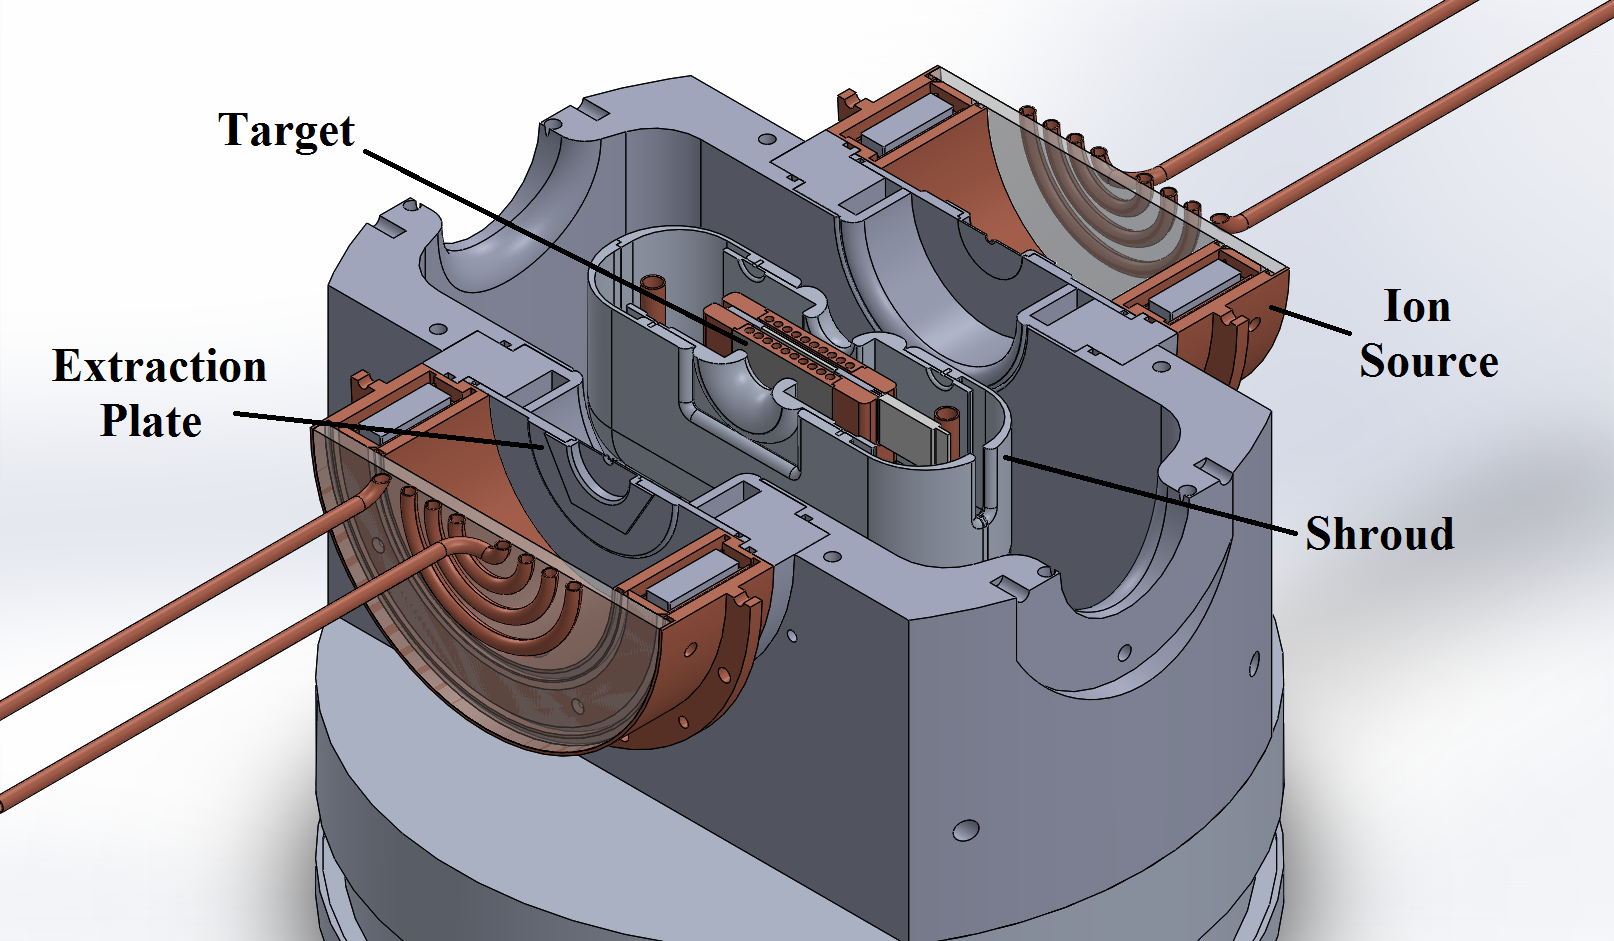
\includegraphics[width=0.5\textwidth]{pics/cutaway}
%DIFDELCMD < 	%%%
\DIFdelendFL \DIFaddbeginFL 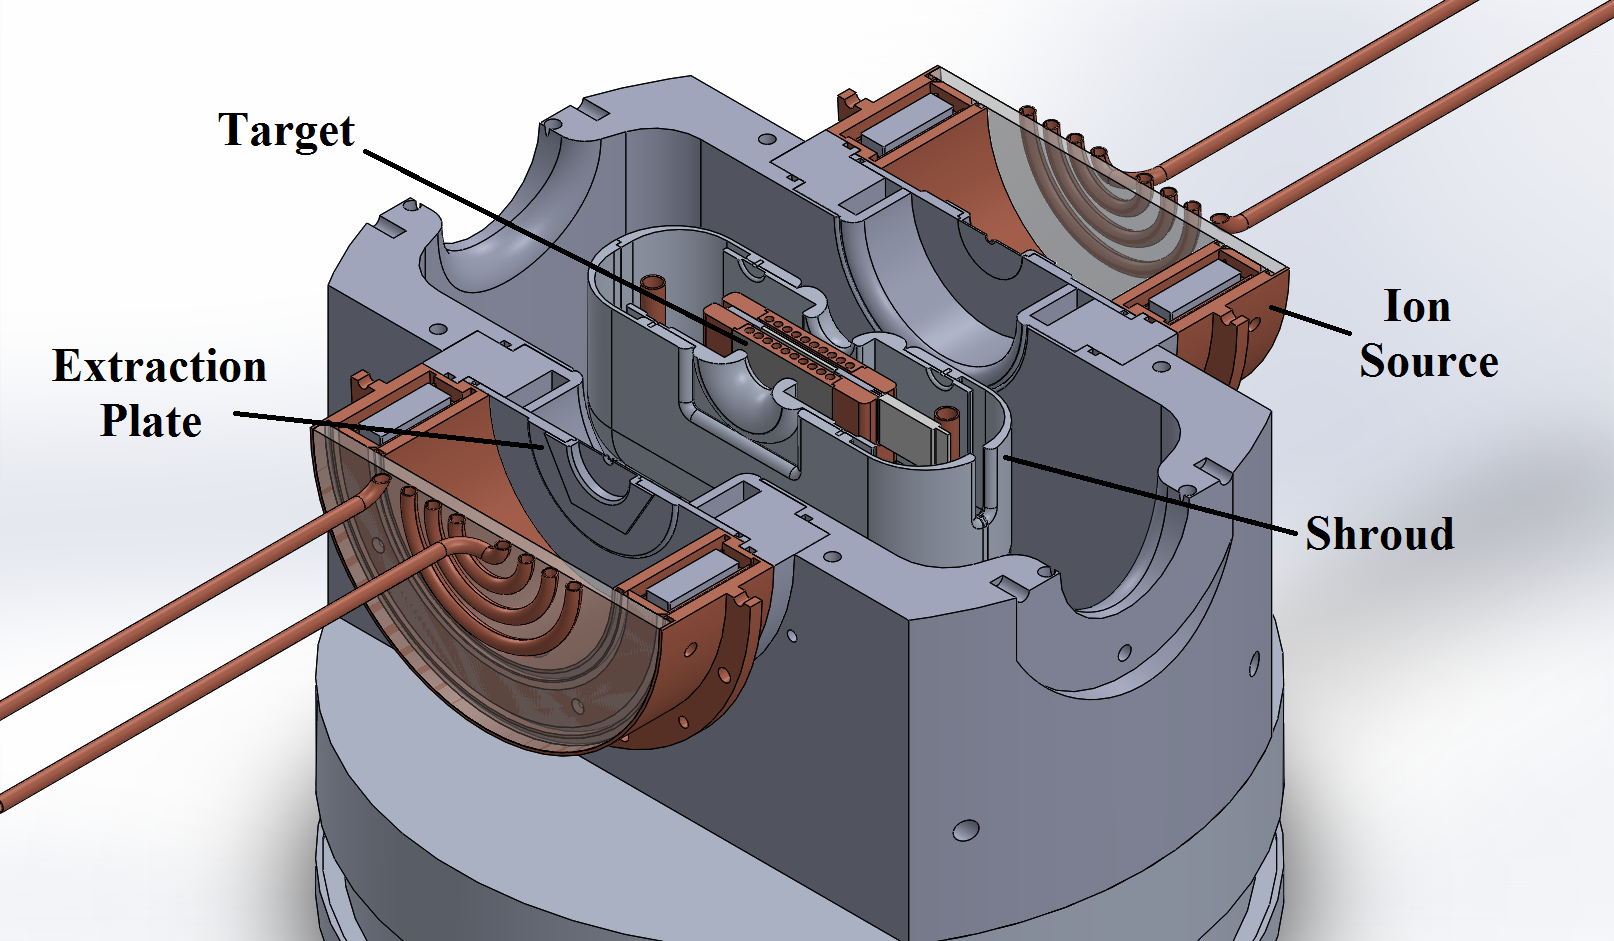
\includegraphics[width=0.7\textwidth]{pics/cutaway}
	\DIFaddendFL \caption{Cross-sectional view of the HFNG exposing the shroud, target, \DIFaddbeginFL \DIFaddFL{extraction plate, }\DIFaddendFL and ion sources. \DIFaddbeginFL \comment{Provide a reference length scale for this schematic, and possibly enlarge it a bit - it's hard to see at its current size, and the design is far more important here than the (n,p) NIM. Also, make sure that this is the ``final/optimized'' design you present later on.}\DIFaddendFL }
	\label{fig:HFNG}
\end{figure}

The target, shown in Figure \ref{fig:new_target}, is \DIFdelbegin \DIFdel{mostly made }\DIFdelend \DIFaddbegin \DIFadd{primarily composed }\DIFaddend of copper due to its excellent thermal conductivity. However, copper does not form hydrides as well as titanium\DIFdelbegin \DIFdel{does \mbox{%DIFAUXCMD
\cite{CRC}
}%DIFAUXCMD
. Therefore, }\DIFdelend \DIFaddbegin \DIFadd{, so }\DIFaddend a thin layer (120 microns) of titanium is \DIFdelbegin \DIFdel{explosion bonded }\DIFdelend \DIFaddbegin \DIFadd{explosion-bonded }\DIFaddend onto the copper structure \DIFaddbegin \DIFadd{to enhance deuteride implantation \mbox{%DIFAUXCMD
\cite{CRC}
}%DIFAUXCMD
}\DIFaddend . The unique design of this target allows for samples to be placed very close to the neutron \DIFdelbegin \DIFdel{emitting spot ($\approx 8 mm$ relative distance), hence }\DIFdelend \DIFaddbegin \DIFadd{production surface ($\approx 8$ mm separation), }\DIFaddend maximizing the neutron flux at the sample location. Active \DIFaddbegin \DIFadd{internal }\DIFaddend cooling with deionized water is \DIFdelbegin \DIFdel{needed in order }\DIFdelend \DIFaddbegin \DIFadd{necessary }\DIFaddend to dissipate the heat load generated by the deuterium beam incident upon the surface of the target. The target is biased at a negative potential (up to -120 kV) in order to extract the positive deuterium ions.

\begin{figure}
	\centering
	\DIFdelbeginFL %DIFDELCMD < 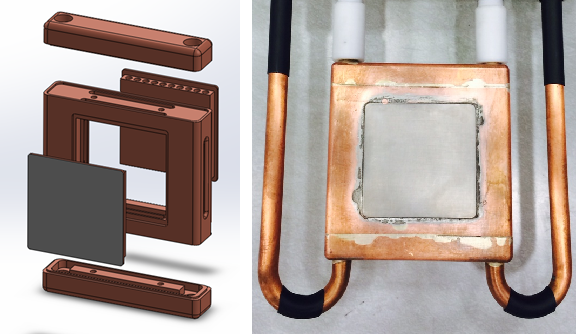
\includegraphics[width=0.5\textwidth]{pics/new_target}
%DIFDELCMD < 	%%%
\DIFdelendFL \DIFaddbeginFL 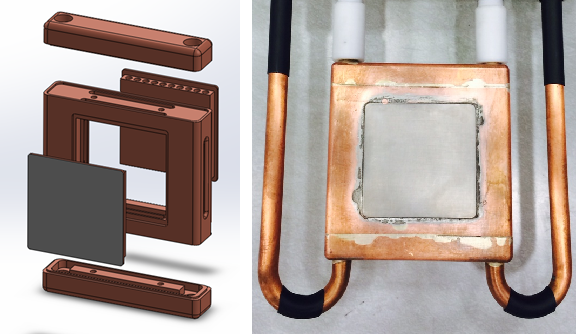
\includegraphics[width=0.6\textwidth]{pics/new_target}
	\DIFaddendFL \caption{Target assembly showing the CAD design of the faceplate and the actual target soldered in place. \DIFaddbeginFL \DIFaddFL{The gray titanium-coated copper production surface is visible in the center of the target, and cooling lines for deionized water are seen on the sides of the target. }\comment{Feel free to modify this, but it needs a bit more explanation of what is visible in the target.  also needs to be enlarged}\DIFaddendFL }
	\label{fig:new_target}
\end{figure}

The target is encased in a shroud electrode biased at an even lower potential ($\Delta V=2.4\ kV$) through an arrangement of diodes in order to reverse the direction of the electric field inside this structure. The circuit diagram is shown in Figure \ref{fig:diodes}. Without a shroud, electrons that are \DIFdelbegin \DIFdel{sputtered off }\DIFdelend \DIFaddbegin \DIFadd{backscattered off of }\DIFaddend the titanium target \DIFdelbegin \DIFdel{after }\DIFdelend \DIFaddbegin \DIFadd{by }\DIFaddend the deuterium ions \DIFdelbegin \DIFdel{impinge on the target }\DIFdelend would experience a repulsive electrostatic force\DIFdelbegin \DIFdel{that would accelerate }\DIFdelend \DIFaddbegin \DIFadd{, accelerating }\DIFaddend them back towards the extraction plate \DIFdelbegin \DIFdel{causing }\DIFdelend \DIFaddbegin \DIFadd{to cause arcing,  }\DIFaddend overheating (or even melting) of surrounding structures, \DIFdelbegin \DIFdel{arcing, }\DIFdelend and a very large flux of bremsstrahlung\DIFdelbegin \DIFdel{X-rays}\DIFdelend . The electric field reversal inside the shroud makes the electrons experience \DIFdelbegin \DIFdel{a force }\DIFdelend \DIFaddbegin \DIFadd{an attractive force which guides them }\DIFaddend back towards the target, \DIFdelbegin \DIFdel{which makes them return to it, hence }\DIFdelend mitigating the issues mentioned above. A detailed discussion of this technique has already been published \cite{electronSup}. 

\begin{figure}
	\centering
	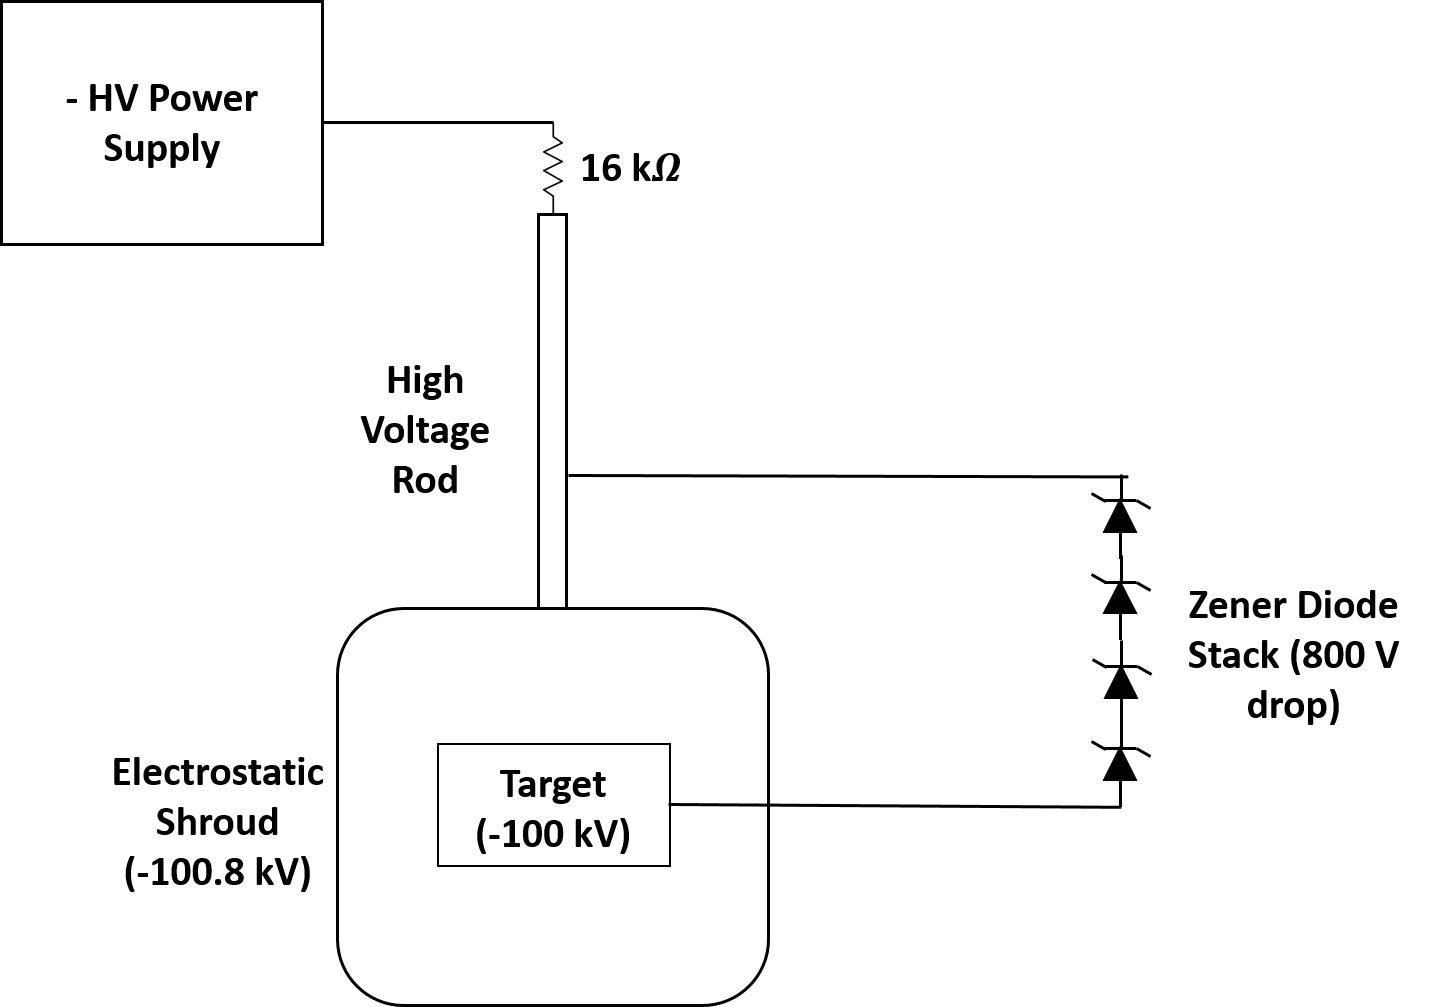
\includegraphics[width=0.7\textwidth]{pics/diodes3}
	\caption{Circuit schematic of the diode assembly\DIFaddbeginFL \DIFaddFL{, for typical operation at a -XXXXX V bias potential}\DIFaddendFL . Note that the voltage differential between the shroud and the target can be varied from 0 to 2.4 kV. \DIFaddbeginFL \comment{I thought we typically run at -120 kV?  Make sure that the values you quote in this diagram are consistent with normal operating conditions.}\DIFaddendFL }
	\label{fig:diodes}
\end{figure}

The \DIFaddbegin \DIFadd{HFNG's internal }\DIFaddend vacuum chamber is evacuated by a scroll pump connected in series with a \DIFdelbegin \DIFdel{turbo-pump}\DIFdelend \DIFaddbegin \DIFadd{turbopump, designed to operate at an internal pressure of XXXXXX  }\comment{List what a typical range of operating pressure is.}\DIFaddend . The scroll pump is oil-free; \DIFdelbegin \DIFdel{this is important as }\DIFdelend \DIFaddbegin \DIFadd{since }\DIFaddend the HFNG produces a \DIFdelbegin \DIFdel{certain amount }\DIFdelend \DIFaddbegin \DIFadd{finite amount (approximately XXXXX uCi / hour of operation) }\DIFaddend of tritium during operation, which readily binds \DIFdelbegin \DIFdel{with oil molecules. }\DIFdelend \DIFaddbegin \DIFadd{to oil molecules, oil-free pumps help minimize dispersible tritium contamination. }\comment{Have we measured what typical tritium levels are produced duirng operation?  nCi / hr?  uCi/hr?  You say that a certain amount is produced, you need to quantify that here.} \DIFaddend Furthermore, a scroll pump can be operated continuously without the risk of backstreaming fluids. \DIFdelbegin %DIFDELCMD < 

%DIFDELCMD < %%%
\DIFdel{A polyethylene structure was constructed that can be assembled around the HFNG to thermalize neutrons for different types of experiments. In general, nuclear reactions of the type $(n,\gamma)$ have higher absorption cross-sections at lower energies.
}%DIFDELCMD < 

%DIFDELCMD < %%%
\DIFdel{There is also an external beam port aligned with the neutron emitting spot of the HFNG in order to perform experiments outside the vault. Some experiments that have been performed using the external beam line include characterization of gamma detectors in a neutron field, and prompt gamma activation analysis of various materials.   
	}%DIFDELCMD < 

%DIFDELCMD < %%%
\DIFdelend The HFNG uses a residual gas analyzer (RGA) system that allows for continuous\DIFdelbegin \DIFdel{/}\DIFdelend \DIFaddbegin \DIFadd{, }\DIFaddend on-line monitoring of the gas composition inside the chamber. It serves as \DIFaddbegin \DIFadd{both }\DIFaddend a leak detector\DIFaddbegin \DIFadd{, }\DIFaddend as well as a reliable indicator of water vapor, which \DIFdelbegin \DIFdel{can cause }\DIFdelend \DIFaddbegin \DIFadd{causes }\DIFaddend a variety of problems during operation.  \DIFaddbegin \comment{Like what?  Briefly describe the problems caused by water vapor.}
	\DIFaddend 

\section{Modeling of	Neutron Yield, Flux and Energy Distribution}
\DIFdelbegin 
% \section{\DIFdel{Neutron Yield, Flux and Energy Distribution}}
	%DIFAUXCMD
\addtocounter{section}{-1}%DIFAUXCMD
%DIFDELCMD < 

%DIFDELCMD < %%%
\DIFdel{The neutron yield has been experimentally determined in an indirect way. Flux measurements via activation foils were carried out (Section 5) and compared to the simulations presented below. Experimental results agree with those of simulations to about 5}%DIFDELCMD < \% %%%
\DIFdel{at the sample holder location. 
}\DIFdelend \DIFaddbegin \DIFadd{In addition to this standard internal irradiation, two alternative modes operation are presently available, providing the possibility to use the HFNG to provide a range of alternative neutron energy distributions for various applications.    A polyethylene structure was constructed and can be assembled around the HFNG to thermalize DD neutrons while maintaining high flux for internal irradiation }\comment{Quote the flux/fluence we see for thermal poly operation.}\DIFadd{. In general, neutron capture cross-sections follow a $1/v$ trend  at lower energies. In this mode of operation, the HFNG can be used as a compact alternative to thermal reactors for  $(n,\gamma)$ activation studies and isotope production.  }\comment{I would insert a picture of both the poly shield, as well as the external beamline cage.  Later on, it would be well worth your while to include neutron spectra for each.  If this article is announcing the possibility to operate the HFNG in these 2 modes, we definitely need to have figures/results describing their characterization.}
\DIFaddend 

\DIFdelbegin \DIFdel{Note that a high yield neutron generator does not directly imply a high flux neutron generator. For instance, there are commercially availableneutron generators with gas targets with DD neutron yields in the order of $10^{11}\ n/s$. However, the flux at any location around the target is several orders of magnitude lower and impractical for our purposes. Moreover, a neutron generator with a solid target but with a large beam spot compared to the sample also suffers from the same effect. In other words, the yield does not scale linearly with the flux when the beam spot increases.  Therefore, the flux is maximized when we operate close to the heat load limit of the target. Hence, a narrow deuterium beam compared to the size of the target is desirable}\DIFdelend \DIFaddbegin \DIFadd{Additionally, there is an external beam port which can be aligned at 90}\degree\ \DIFadd{($\approx$2.45 MeV neutrons) with respect to the production surface  of the HFNG in order to perform experiments outside the vault. }\comment{Correct me if I'm wrong, but wouldnt it be aligned with the 90-degree neutron production angle?  The neutrons are emitted in 4$\pi$, but mostly forward focused, so the beam port should just let through whatever solid angle it subtends?  Doubel check the energies I list here.} \DIFadd{This port is connected to a shielded beam dump and allows for both collimated beams of fast neutrons, as well as a thermal spectrum, using a polyethylene plug in the beam port. A number of experiments  have already been performed using the external beam line, including characterization of gamma detectors in a neutron field, and prompt gamma activation analysis of various materials, with more planned for the future}\DIFaddend .   

\DIFaddbegin \comment{I provided a starting point, but for both the thermal shield and the external beam line, you need to explain WHY they are useful, not just list that they exist. }


	
	

\comment{The text starting off this section \enquote{The neutron yield has been experimentally determined...} isn;t appropriate to start off a section, as it is more of a conclusion / result.  I moved it to the conclusions instead. }


	
\DIFaddend \subsection{Neutron Yield Analysis}

\DIFdelbegin \DIFdel{Some }\DIFdelend \DIFaddbegin \DIFadd{At the ion energy specified by the bias voltage, a fraction }\DIFaddend of the accelerated deuterons do not undergo \DIFdelbegin \DIFdel{fusion reactions at the energy specified by the voltage differential between the target and the plasma electrode }\DIFdelend \DIFaddbegin \DIFadd{DD fusion }\DIFaddend due to two main processes: 1) deuterons slow down as they traverse the target volume before a fusion reaction occurs, and 2) the deuterium \DIFaddbegin \DIFadd{ion }\DIFaddend beam is not purely monatomic, which also lowers the interaction energy \DIFaddbegin \comment{Not sure what you mean by ``lowers the interaction energy.'' Please explain and reword.}\DIFaddend . Both of these processes result in a lower neutron \DIFdelbegin \DIFdel{output }\DIFdelend \DIFaddbegin \DIFadd{yield }\DIFaddend due to the fact that the DD fusion cross-section decreases with decreasing \DIFdelbegin \DIFdel{interaction energy. The slowing  down }\DIFdelend \DIFaddbegin \DIFadd{deuteron ion energy. This slowing  }\DIFaddend process can be described using data for the energy loss per unit distance (stopping power) of deuterons in titanium \cite{SRIM}. \DIFdelbegin \DIFdel{Moreover}\DIFdelend \DIFaddbegin \DIFadd{Additionally}\DIFaddend , the deuterium beam is composed of monatomic \DIFdelbegin \DIFdel{, diatomic}\DIFdelend \DIFaddbegin \DIFadd{(D$^+$), diatomic (D$_2^+$)}\DIFaddend , and triatomic \DIFaddbegin \DIFadd{(D$_3^+$) }\DIFaddend ion species. \DIFdelbegin \DIFdel{The heavier  the }\DIFdelend \DIFaddbegin \DIFadd{For heavier  }\DIFaddend species, the \DIFdelbegin \DIFdel{lower the }\DIFdelend final energy they achieve for a given target potential \DIFaddbegin \DIFadd{is lower}\DIFaddend . For example, molecular \DIFaddbegin \DIFadd{(diatomic) }\DIFaddend deuterium accelerated to 100 keV will share this energy equally between the two deuterium nuclei\DIFdelbegin \DIFdel{i.e. }\DIFdelend \DIFaddbegin \DIFadd{, }\emph{\DIFadd{i.e.}}\DIFadd{, each ion has an energy of }\DIFaddend 50 keV\DIFdelbegin \DIFdel{each}\DIFdelend . For RF ion sources, the deuterium is \DIFdelbegin \DIFdel{mostly monatomic. However}\DIFdelend \DIFaddbegin \DIFadd{strongly monatomic, however}\DIFaddend , the exact composition is, for the most part, a function of the RF power. \DIFdelbegin \DIFdel{Similar ion sources have been studied \mbox{%DIFAUXCMD
\cite{multicusp2}
}%DIFAUXCMD
and these reports indicate }\DIFdelend \DIFaddbegin \comment{Why?  Explain, and provide sources.}  \DIFadd{Similar ion source designs have been characterized \mbox{%DIFAUXCMD
\cite{multicusp2}
}%DIFAUXCMD
,  indicating }\DIFaddend that at 1200 W (standard for the HFNG), the ratios between the three species are approximately 0.65:0.25:0.10, respectively. Even though RF ion sources produce mostly monatomic deuterium ions, the recombination process is significantly affected by the contact material.
\DIFaddbegin \comment{Provide a source!} \DIFaddend Insulators are better at hindering recombination, while conductors such as copper have much higher recombination coefficients.   \DIFaddbegin \comment{Provide a source!} 
\DIFaddend 

The neutron yield can be approximated based on an analytical approach outlined in \cite{CRC}\DIFaddbegin \DIFadd{, }\DIFaddend together with empirical data for the stopping power ($dE/dx$) of deuterons in titanium, the cross-section for the neutron-producing \DIFdelbegin \DIFdel{reaction in Equation \ref{eq:reactionDD}}\DIFdelend \DIFaddbegin \DIFadd{DD reaction}\DIFaddend , the fraction of different deuterium species in the ion source, and the deuterium-to-titanium ratio in the self-loaded target, which was taken to be one-to-one for a conservative estimate. \DIFaddbegin \comment{Is this  a mass ratio?  Atom ratio?  Specify.} \DIFaddend Equation \ref{eq:yield} was used to \DIFdelbegin \DIFdel{calculate }\DIFdelend \DIFaddbegin \DIFadd{estimate }\DIFaddend the neutron yield as a function of deuteron energy \DIFaddbegin \DIFadd{($E_d$)}\DIFaddend , where $\phi_d$ is the deuteron flux (\DIFdelbegin \DIFdel{$cm^{-2}s^{-1}$}\DIFdelend \DIFaddbegin \DIFadd{cm$^{-2}$s$^{-1}$}\DIFaddend ) incident on the target, $n_d$ is the number density of deuterons in the target (\DIFdelbegin \DIFdel{$cm^{-3}$}\DIFdelend \DIFaddbegin \DIFadd{cm$^{-3}$}\DIFaddend ) when saturated, $\sigma(E_d)$ is the cross section for the DD neutron-producing reaction \DIFaddbegin \DIFadd{(mb?)}\DIFaddend , and $dE/dx(E_d)$ is the energy loss per unit distance in titanium. Note that the lower limit of integration is taken to be zero since the Q-value of the reaction is positive. \DIFdelbegin \DIFdel{The yield  calculated with this equation }\DIFdelend \DIFaddbegin \DIFadd{This estimated yield  }\DIFaddend is an input for the MCNP \cite{MCNP} model, which calculates the neutron flux per source \DIFdelbegin \DIFdel{particle. 
}\DIFdelend \DIFaddbegin \DIFadd{deuteron. 
}

\comment{If the flux profile comes from MCNP, and you use the resulting yield as MCNP input, isn;t that a circular system?  This needs a lot of work to clarify what you refer to.}


\comment{Where do you get each of these quantities from?  Please specify.  I assume flux comes from MCNP, cross section from Liskien-Paulsen, stopping power from SRIM.  Cite each here after you mention them, for clarity.}

\comment{How do you determine when the the target is saturated? and how you measure the number density at that point?  REALLY elaborate on that here.}

\DIFaddend This approach agrees with experiments relatively well, as discussed in the last section.  
\DIFaddbegin \comment{You can't just say ``relatively well'' - provide a concrete number, and consider moving discussion of results to later on, since you are here describing the input of modeling, not necessarily results yet.}
\DIFaddend 

\begin{equation} \label{eq:yield}
Y(E_d)=\phi_d n_d \int_{0}^{E_{max}} \frac{\sigma(E_d)}{dE/dx(E_d)}dE_d
\end{equation}

	
\subsection{Neutron Flux and Energy Distribution}

The kinematics of the \DIFaddbegin \DIFadd{2-body }\DIFaddend interaction between deuterons results in a \DIFaddbegin \DIFadd{well-characterized }\DIFaddend variation of neutron energy as a function of angle in the lab frame \DIFdelbegin \DIFdel{. From energy and momentum conservation, the energy of the emitted neutron varies as shown }\DIFdelend \DIFaddbegin \comment{Provide source!  Likely Liskien-Paulsen}\DIFadd{. This neutron energy-angle variation is seen for a range of ion energies }\DIFaddend in Figure \ref{fig:energy_dist}\DIFdelbegin \DIFdel{. Note that the variation can be }\DIFdelend \DIFaddbegin \DIFadd{, clearly displaying that this variation is }\DIFaddend quite significant. For instance, at zero deuteron incident kinetic energy, the energy of the emitted neutron is 2.45 MeV, while at 100 keV, the maximum is close to 2.8 MeV. The apparent violation of  \DIFdelbegin \DIFdel{the }\DIFdelend conservation of energy  \DIFdelbegin \DIFdel{principle }\DIFdelend is accounted for by the redistribution of the total \DIFdelbegin \DIFdel{available }\DIFdelend \DIFaddbegin \DIFadd{excitation }\DIFaddend energy (Q-value plus incident deuteron energy) between the \DIFdelbegin \DIFdel{He-3 }\DIFdelend \DIFaddbegin \DIFadd{$^3$He }\DIFaddend nucleus and the neutron. 

\begin{figure}
	\centering
	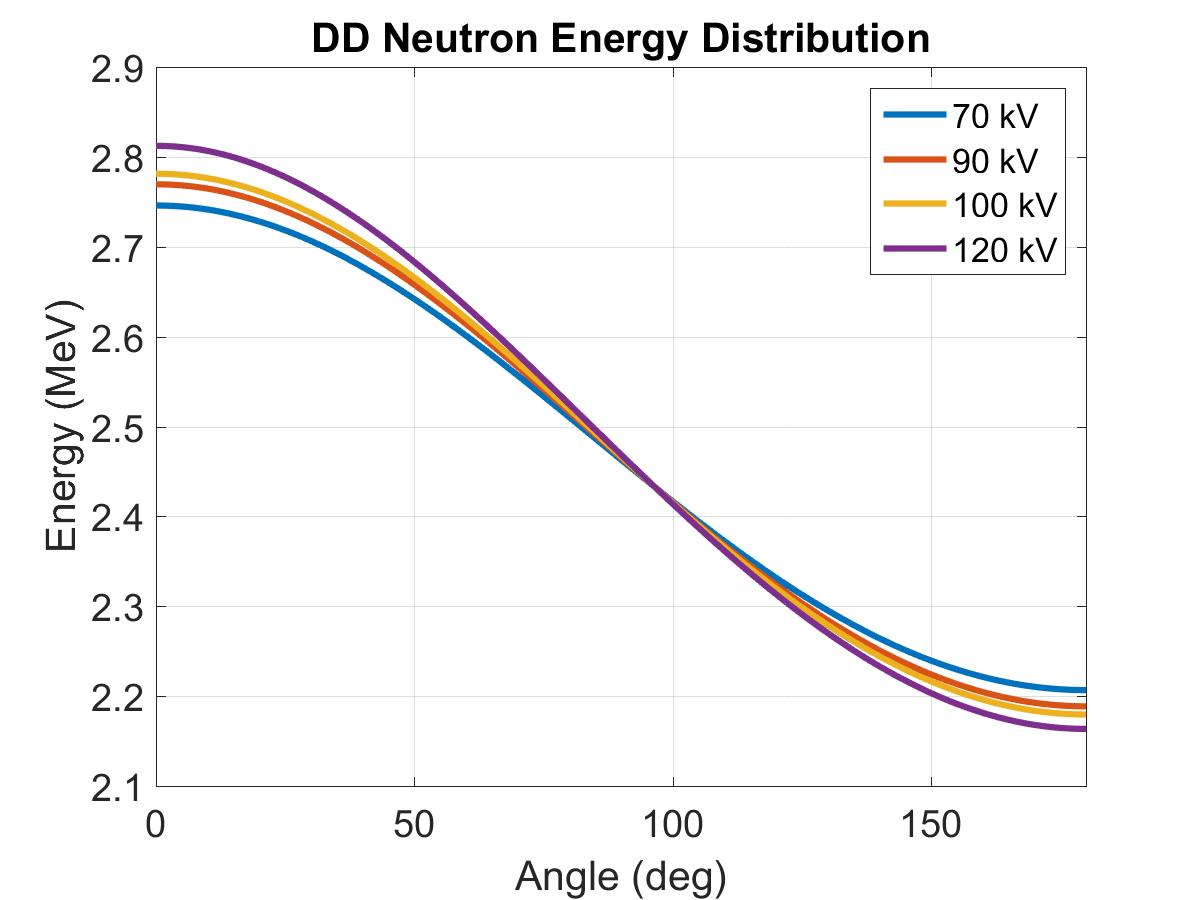
\includegraphics[width=0.7\textwidth]{pics/energy_dist}
	\caption{Neutron energy in the lab system as a function of angle. \DIFaddbeginFL \DIFaddFL{With increasing ion energy, a wider spread in neutron energy is seen over the 0-180}\degree\ \DIFaddFL{range. }\comment{If this is Liskien-Paulsen data, it needs to be cited here in teh caption, too.}\DIFaddendFL }
	\label{fig:energy_dist}
\end{figure}

The energy spectrum changes slightly as the neutron travels through the target\DIFdelbegin \DIFdel{. Therefore, }\DIFdelend \DIFaddbegin \DIFadd{, }\comment{What do you mean it ``changes slightly''?  Does it broaden? Dampen? Be specific. } \DIFadd{leading to }\DIFaddend different empirical correlations  \DIFdelbegin \DIFdel{were found }\DIFdelend for thin and thick targets \cite{CRC}. \DIFaddbegin \comment{Need to define thin vs thick target.  Give ranges in mg/cm$^2$.} \DIFaddend The angular distribution is well-fitted with an expansion in Legendre polynomials, as shown in Equation \ref{eqn:energDist}. Note that this equation is valid for DD and DT reactions below \DIFdelbegin \DIFdel{$500\ keV$ for both , }\DIFdelend \DIFaddbegin \DIFadd{$500$ keV deuteron energy for both }\DIFaddend thin and thick targets. 

\begin{equation}
E_n(E_d,\theta)=E_0+\sum_{i=1}^{n}E_i cos^i \theta
\label{eqn:energDist}
\end{equation}

The coefficients $E_i$ were determined for a few energy values \DIFdelbegin \DIFdel{only }\DIFdelend \DIFaddbegin \DIFadd{of deuteron energy }\DIFaddend \cite{CRC}. Therefore, they were interpolated in this code using a cubic spline \DIFdelbegin \DIFdel{for any }\DIFdelend \DIFaddbegin \DIFadd{to be applicable for a wider range of }\DIFaddend desired energy. \DIFdelbegin %DIFDELCMD < 

%DIFDELCMD < %%%
\DIFdelend \DIFaddbegin \comment{Which code are you refrring to?  This is the first tiem you mention any code.  Please explain in-text.} \DIFaddend Furthermore, the neutron yield is also dependent on the emitted angle, and DD neutrons exhibit a larger anisotropy than DT neutrons. \DIFdelbegin \DIFdel{The highest }\DIFdelend \DIFaddbegin \comment{Why?  Explain and provide sources.} \DIFadd{The }\DIFaddend yield in this \DIFdelbegin \DIFdel{kind of }\DIFdelend \DIFaddbegin \DIFadd{design of DD }\DIFaddend neutron generators is \DIFdelbegin \DIFdel{along the deuteron beam direction }\DIFdelend \DIFaddbegin \DIFadd{forward-focused, with the maximum yield in the direction of the incident deuteron beam  }\DIFaddend ($0^\circ$). The relative yield, defined as the total yield normalized to that at $90^{\circ}$, can be described by Equation~\ref{eqn:angDist}\DIFdelbegin \DIFdel{. This equation comes from a best fit }\DIFdelend \DIFaddbegin \DIFadd{, a best-fit }\DIFaddend model of the available data \cite{CRC}.

\begin{equation}
\frac{Y(\theta)}{Y(90^{\circ})}=A_0+\sum_{i=1}^{n}A_i cos^i \theta
\label{eqn:angDist}
\end{equation}

\DIFaddbegin \comment{Why do you choose to normalize to the 90\degree\ yield?  Please explain, and, if its an arbitrary choice, describe why you chose 90\degree\ over, say, 0\degree.}

\DIFaddend The coefficients $A_i$ were interpolated using a cubic spline for \DIFdelbegin \DIFdel{any desired voltage value. Figure~\ref{fig:yield} shows the relative yield distribution }\DIFdelend \DIFaddbegin \DIFadd{various deuteron energies, with the resulting relative yield distributions }\DIFaddend in the lab frame  \DIFdelbegin \DIFdel{for various voltages}\DIFdelend \DIFaddbegin \DIFadd{shown in Figure~\ref{fig:yield}}\DIFaddend .

\begin{figure}[H]
	\begin{center}
		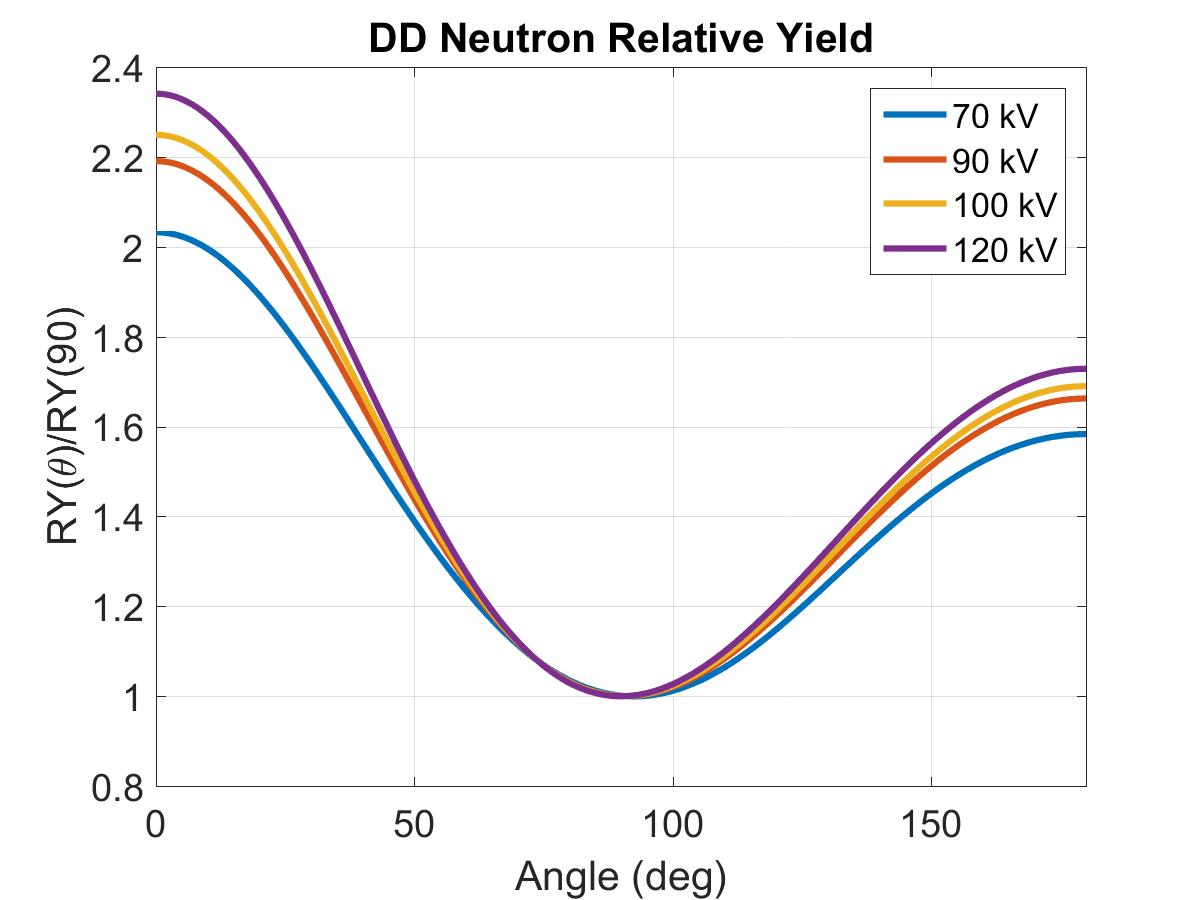
\includegraphics[width=0.7\textwidth]{pics/rel_yield} 
		\caption{Relative neutron yield for different accelerating voltages\DIFdelbeginFL \DIFdelFL{(DD reactions)}\DIFdelendFL . \DIFaddbeginFL \DIFaddFL{Neutron yield becomes increasingly more pronounced with larger voltage at forward and backward angles. }\comment{In figure captions, you need to provide more than a description of what is in the figure, give commentary on its significance also.  Also, you use RY($\theta$) on the axis label here, but Y($\theta$) in \ref{eqn:angDist} - be consistent. }\DIFaddendFL }
		\label{fig:yield}
	\end{center}
\end{figure}

\DIFdelbegin \DIFdel{We developed an }\DIFdelend \DIFaddbegin \comment{Need to specifiy the version of MCNP you used, and cite its tech doc.}

\DIFadd{An }\DIFaddend MCNP model of the generator and surrounding structures \DIFdelbegin \DIFdel{. The neutron source  is }\DIFdelend \DIFaddbegin \DIFadd{was developed, with the neutron source  }\DIFaddend modeled according to experimental data obtained from \cite{Cross_sections}. The \DIFdelbegin \DIFdel{main }\DIFdelend \DIFaddbegin \DIFadd{primary }\DIFaddend purpose of such a model is to obtain the flux and energy distributions at different irradiation locations. The titanium target is considered to be ``thick'' in the sense that all accelerated deuterons either interact or stop within the target; deuterons penetrate the target a maximum of just under 1 micron at 120 kV \DIFaddbegin \comment{You need a source for that}\DIFaddend , while the titanium layer is several hundred \DIFdelbegin \DIFdel{micrometers }\DIFdelend \DIFaddbegin \DIFadd{microns }\DIFaddend thick. The types of neutron sources considered in the MCNP model were point-like, disk \DIFaddbegin \comment{Specify diameter}\DIFaddend , and Gaussian shaped \DIFaddbegin \comment{Specify centroid and 1-$\sigma$ width}\DIFaddend , with the latter being the \DIFdelbegin \DIFdel{more }\DIFdelend \DIFaddbegin \DIFadd{most }\DIFaddend accurate representation of the actual source (single-hole extraction) \DIFdelbegin \DIFdel{. The code developed }\DIFdelend \DIFaddbegin \comment{What are you basing this ``most accurate'' claim on?  Benchmarking?  Back up your claim.}\DIFadd{. The model  }\DIFaddend allows for different input parameters to be modified according to the experiment being performed. \DIFdelbegin \DIFdel{Such }\DIFdelend \DIFaddbegin \DIFadd{These tunable }\DIFaddend parameters include the acceleration voltage, the deuterium ion current, the atomic deuterium ion fraction in the plasma, the beam diameter, and the Gaussian profile of the beam. \DIFdelbegin \DIFdel{These results }\DIFdelend \DIFaddbegin \DIFadd{The resulting neutron energy distributions for each source definition }\DIFaddend are shown in Figure \ref{fig:source_definitions}. Note that there is no significant difference among the three different source definitions\DIFdelbegin \DIFdel{for this specific case. }\DIFdelend \DIFaddbegin \DIFadd{. }\comment{to back up this claim, you really should provide a residuals plot, since at the current scaling of the figure, you can't look for any systematic differences.} \DIFaddend However, if the irradiation location or the size of the samples change, it is important to re-check that these definitions \DIFdelbegin \DIFdel{agree.  }\DIFdelend \DIFaddbegin \DIFadd{are still consistent.  }\comment{Why would you expect them to agree?}   
\DIFaddend 

\begin{figure}
	\centering
	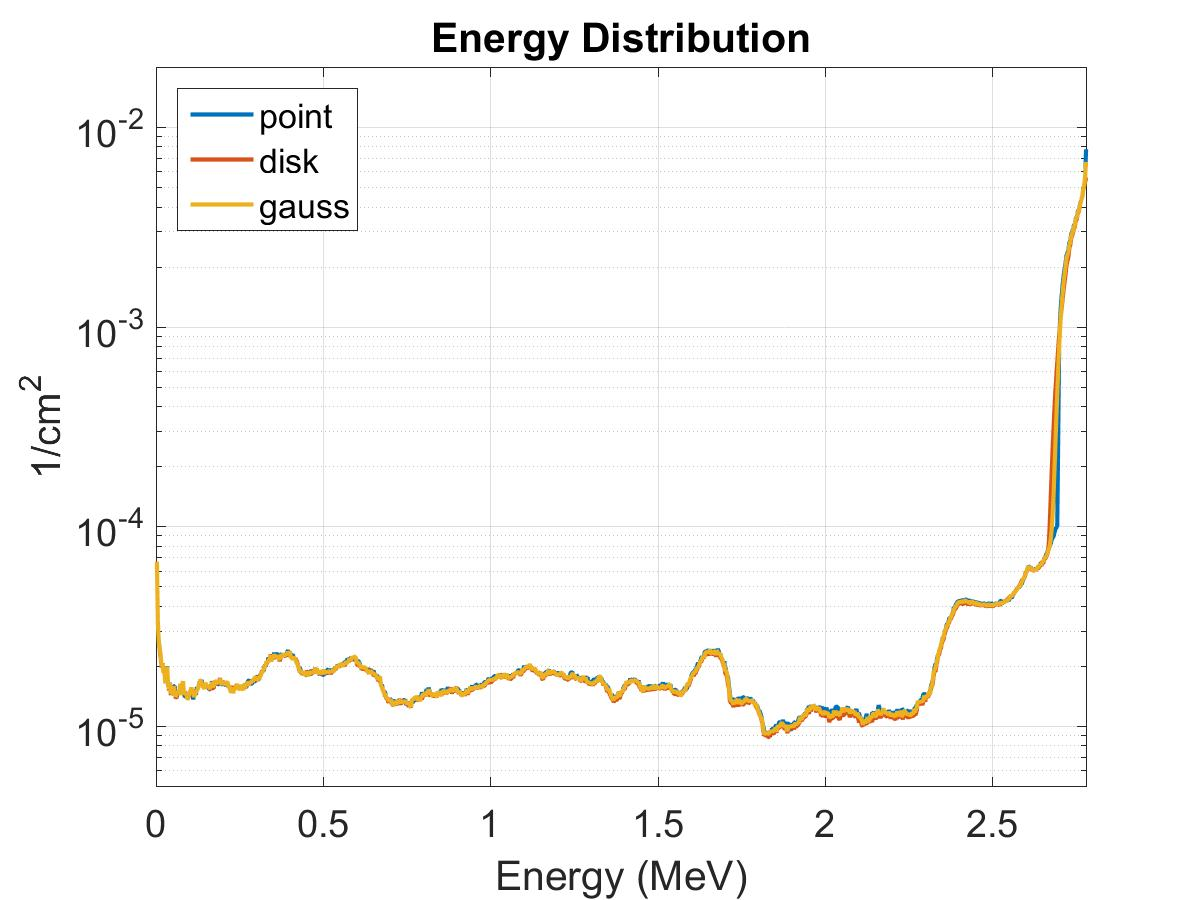
\includegraphics[width=0.7\textwidth]{pics/comp_sources_log}
	\caption{\DIFdelbeginFL \DIFdelFL{MCNP simulations for different source definitions in terms of }\DIFdelendFL \DIFaddbeginFL \DIFaddFL{MCNP-simulated }\DIFaddendFL energy \DIFdelbeginFL \DIFdelFL{distribution }\DIFdelendFL \DIFaddbeginFL \DIFaddFL{distributions  }\DIFaddendFL at the center of the sample holder location \DIFaddbeginFL \DIFaddFL{for different source definitions}\DIFaddendFL . \DIFdelbeginFL \DIFdelFL{Units }\DIFdelendFL \DIFaddbeginFL \DIFaddFL{Flux units }\DIFaddendFL on the y-axis are normalized per source neutron. \DIFaddbeginFL \comment{Your y-axis has no label, the units alone are insufficient. For the disk and Gaussian sources, you have to provide the parameters you used for each sources - diameter, and centroid and width, respectively. In the legend, capitalize the entries, and don't abbreviate Gaussian.  Also, you should comment on what causes the feature near 1.7 MeV.}\DIFaddendFL }
	\label{fig:source_definitions}
\end{figure}

\DIFaddbegin \comment{Make sure to comment on the paucity of thermal neutrons in this spectrum, and the importance of this for preventing unwanted (n,$\gamma$) contamination. You'll want to point back to this later in your results.}


\DIFaddend In order to take advantage of the variation of neutron energy as a function of angle, \DIFdelbegin \DIFdel{a }\DIFdelend \DIFaddbegin \DIFadd{an }\DIFaddend L-shaped sample holder\DIFdelbegin \DIFdel{was designed and machined so that }\DIFdelend \DIFaddbegin \DIFadd{, shown in Figure \ref{fig:L_holder}, was designed so that multiple }\DIFaddend samples can be \DIFdelbegin \DIFdel{located in such a way as }\DIFdelend \DIFaddbegin \DIFadd{loaded  }\DIFaddend to span neutron energies between 2.4 - 2.8 MeV at 100 kV extraction voltage\DIFdelbegin \DIFdel{, as shown in Figure \ref{fig:L_holder}}\DIFdelend . This arrangement is particularly interesting for cross section measurements\DIFaddbegin \DIFadd{, as it permits measurement }\DIFaddend at different neutron energies \DIFaddbegin \DIFadd{in a single irradiation}\DIFaddend . It has been used for \DIFdelbegin \DIFdel{$^{35}Cl(n,p)$ and $^{35}Cl(n,\alpha)$ }\DIFdelend \DIFaddbegin \DIFadd{$^{35}$Cl(n,p) and $^{35}$Cl(n,$\alpha)$ }\DIFaddend reaction cross section measurements. \DIFaddbegin \comment{Check with Batch to see if he has anything we can cite for now, even if its just a conferenece talk.} \DIFaddend The size of the energy window depends on the size of the sample, and MCNP simulations should be performed in order to \DIFdelbegin \DIFdel{quantify }\DIFdelend \DIFaddbegin \DIFadd{estimate }\DIFaddend this energy spread. The sample slot located at \DIFdelbegin \DIFdel{$98^{\circ}$ }\DIFdelend \DIFaddbegin \DIFadd{$98.1^{\circ}$ }\DIFaddend allows for a ``clean'' neutron beam, which means that there is virtually no structural material in between the sample and the neutron \DIFdelbegin \DIFdel{emitting spot}\DIFdelend \DIFaddbegin \DIFadd{production surface}\DIFaddend . This arrangement allows for a more narrow energy distribution \DIFaddbegin \DIFadd{(since no scattering occurs on structural materials)}\DIFaddend , but at the expense of a reduced neutron flux due to the $1/r^2$ dependence and the kinematics of the reaction \DIFaddbegin \DIFadd{yield}\DIFaddend , as shown in Figure \ref{fig:yield}. 


\begin{figure}
	\centering
	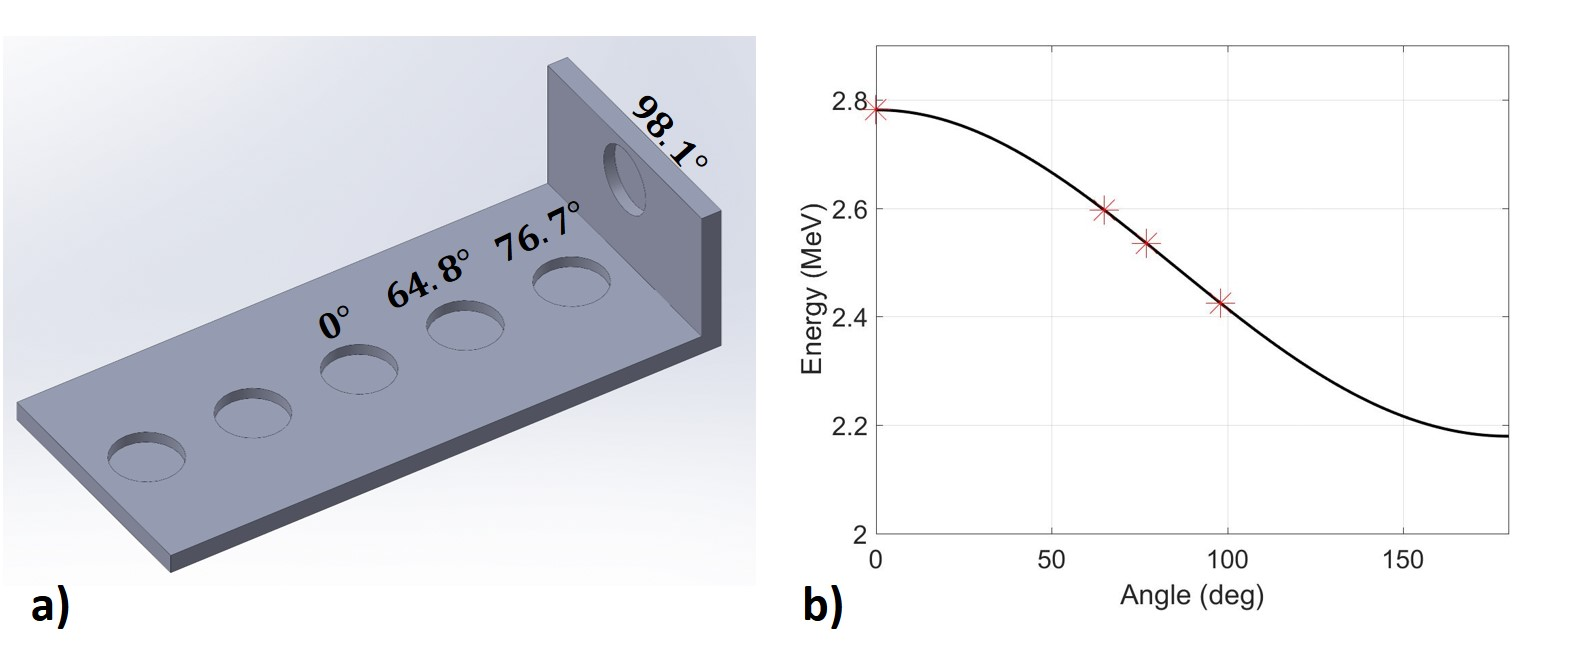
\includegraphics[width=1\textwidth]{pics/L_holder_ang2}
	\caption{Sample holder that allows for irradiation of samples at different neutron energies. The \DIFdelbeginFL \DIFdelFL{values }\DIFdelendFL \DIFaddbeginFL \DIFaddFL{energies }\DIFaddendFL shown correspond to a 100 kV extraction voltage. \DIFaddbeginFL \comment{For teh leftmost two slots, it looks like they shoudl also be 54.8\degree\ and 76.7\degree\ positions, but you should label them such for clarity. Also, provide (eitehr  in the caption or drawn on with an arrow), dimensions for the holder - l x w x h, and sample slot diameter. In subfigure b), make the energy points larger and bolder. }\DIFaddendFL }
	\label{fig:L_holder}
\end{figure}

\section{Ion Beam Extraction Analysis}

The deuterium beam is extracted from the plasma electrode of the ion source through either \DIFdelbegin \DIFdel{one }\DIFdelend \DIFaddbegin \DIFadd{a single }\DIFaddend or multiple apertures. The configuration and design of such an extraction mechanism largely determines the beam profile. Precise knowledge and control of the ion optics is necessary in order to 1) achieve a uniform beam profile on the surface of the target and 2) prevent the localized temperature \DIFdelbegin \DIFdel{to reach $\sim 200^{\circ}\ C$ }\DIFdelend \DIFaddbegin \DIFadd{from reaching $\approx 200^{\circ}\ C$ }\DIFaddend \cite{AANG}. The first requirement ensures that the resulting neutron flux is also uniform over the sample to be irradiated, which is essential for  \DIFdelbegin \DIFdel{several }\DIFdelend experiments such as the irradiation of geological samples \cite{geochron}. The second requirement has to do with the fact that \DIFaddbegin \DIFadd{implanted }\DIFaddend deuterium degases from titanium \DIFdelbegin \DIFdel{around this temperature}\DIFdelend \DIFaddbegin \DIFadd{at XXXXX  }\comment{Provide actual degassing temperature value here, and provide citation for it. You use 230 C later on, but 200 C.  Which is it?  Be consistent.}\DIFaddend , which results in a lower neutron output. Moreover, if the heat load surpasses a certain value determined by the specific target configuration, the target can be eroded and destroyed. \DIFaddbegin \comment{Give a ballpark value of this criticla failure heat load.}
\DIFaddend 

The optimum beam spot \DIFdelbegin \DIFdel{size }\DIFdelend \DIFaddbegin \DIFadd{diameter }\DIFaddend varies according to the application of the neutron generator. For example, a very small spot size \DIFaddbegin \DIFadd{(approximately XXX - YYY mm) }\comment{fill in values.  When would larger spot size be advantageous?} \DIFaddend is needed for fast neutron imaging \DIFdelbegin \DIFdel{because }\DIFdelend \DIFaddbegin \DIFadd{as }\DIFaddend it enhances the sharpness of the image \cite{adams}. However, this requirement limits the beam current the target can handle, which\DIFaddbegin \DIFadd{, }\DIFaddend in turn, limits the neutron yield at a given acceleration voltage. The HFNG \DIFdelbegin \DIFdel{allows }\DIFdelend \DIFaddbegin \DIFadd{is designed }\DIFaddend for a variety of \DIFdelbegin \DIFdel{(exchangeable ) }\DIFdelend \DIFaddbegin \DIFadd{exchangeable }\DIFaddend extraction plate designs\DIFdelbegin \DIFdel{that }\DIFdelend \DIFaddbegin \DIFadd{, which }\DIFaddend result in different beam profiles depending on the application. Extensive analysis and modeling \DIFdelbegin \DIFdel{was }\DIFdelend \DIFaddbegin \DIFadd{were }\DIFaddend performed for a single extraction aperture of 0.262 cm in diameter and a multiple-hole extraction plate. \DIFaddbegin \comment{Describe the process that led to the selection of this diameter.}
\DIFaddend 

A flat plasma meniscus at extraction is desired in order to achieve a uniform beam profile \cite{CoryThesis}. However, precise modeling of the plasma meniscus is complicated due to \DIFdelbegin \DIFdel{all the variables involved and the }\DIFdelend \DIFaddbegin \DIFadd{the complex geometry of the HFNG and }\DIFaddend imperfect fidelity of plasma physics simulations (\DIFdelbegin \DIFdel{specially }\DIFdelend \DIFaddbegin \DIFadd{especially }\DIFaddend near plasma boundaries). Moreover, slight changes in electron temperature and ion density in the plasma \DIFaddbegin \DIFadd{significantly }\DIFaddend affect the shape of the plasma meniscus, as determined by Bohm's Equation \cite{plasma}. \DIFdelbegin \DIFdel{Nevertheless, as }\DIFdelend \DIFaddbegin \comment{You refer to the Bohm equation here, include it in the text.} \DIFadd{As }\DIFaddend the diameter of the extraction aperture decreases, the effects of the plasma meniscus \DIFaddbegin \DIFadd{shape }\DIFaddend on the resulting beam profile are greatly reduced, \DIFdelbegin \DIFdel{and }\DIFdelend \DIFaddbegin \DIFadd{to the point that, }\DIFaddend at very small (\DIFdelbegin \DIFdel{$\sim 1\ mm$}\DIFdelend \DIFaddbegin \DIFadd{$\approx 1\ mm$}\DIFaddend ) apertures, the extracted beam is barely affected by focusing or defocusing effects\DIFdelbegin \DIFdel{due to the shape of the plasma meniscus}\DIFdelend .   

The finite-element software package \DIFdelbegin \DIFdel{Comsol Multiphysics was used in order }\DIFdelend \DIFaddbegin \DIFadd{COMSOL Multiphysics }\comment{Corrected capitalization to match the company. Please specify version and provide citation.} \DIFadd{was used }\DIFaddend to simulate the ion beam trajectory for a single extraction aperture nozzle of 0.262 cm diameter and a 19-hole extraction electrode (each 1 mm \DIFdelbegin \DIFdel{id }\DIFdelend \DIFaddbegin \DIFadd{internal }\DIFaddend diameter), as shown in Figure \ref{fig:single_vs_mult}. \DIFaddbegin \comment{Again, you need to explain where the choice of these diameters and number of holes came from.  Iterative modeling> Cory's thesis?  Please specify.} \DIFaddend The geometry of the setup is \DIFdelbegin \DIFdel{accurately represented }\DIFdelend \DIFaddbegin \DIFadd{consistently represented in COMSOL, }\DIFaddend as it is imported from \DIFdelbegin \DIFdel{a CAD program}\DIFdelend \DIFaddbegin \DIFadd{the CAD designs used for machining the HFNG's structural components}\DIFaddend . The assumptions built into the simulations are as follows\DIFdelbegin \DIFdel{.
}\DIFdelend \DIFaddbegin \DIFadd{:
}\DIFaddend 

1) Ions are extracted from a flat plasma meniscus, which is a reasonably good assumption because of the small size of the extraction aperture and when operated near the Child-Langmuir limit. \DIFaddbegin \comment{Need a citation for Child-Langmuir law.}
\DIFaddend 

2) All ions are born with the same speed and with a perpendicular velocity to the surface of the plasma. Even though the energy of the ions in the plasma follows \DIFdelbegin \DIFdel{the }\DIFdelend \DIFaddbegin \DIFadd{a }\DIFaddend Maxwell-Boltzmann distribution, this assumption encompasses the overall behavior of the beam as it travels to the target. 

Figure \ref{fig:beam_spread} shows the electric potential and the simulated particle trajectories at a target bias and beam current of 100 kV and 1.4 mA, respectively. Note in Figure \ref{subfig:beam_spread} that the equipotential lines near extraction result in a slightly focusing field. This is due to the \DIFdelbegin \DIFdel{geometry of our setup that required }\DIFdelend \DIFaddbegin \DIFadd{HGNG geometry, which requires that }\DIFaddend the ion source to be recessed back a certain distance in order to achieve the desired current density, reduce the maximum electric field in that region, and allow for the beam to spread so the heat flux on the surface \DIFdelbegin \DIFdel{becomes acceptable .
}\DIFdelend \DIFaddbegin \DIFadd{remains within acceptable limits of approximately XXXX.  }\comment{Clarify what ``that region'' refers to, and giev a ballpark heat limit.}
\DIFaddend 

\begin{figure}
	\centering
	\subfloat[\label{subfig:beam_spread}]{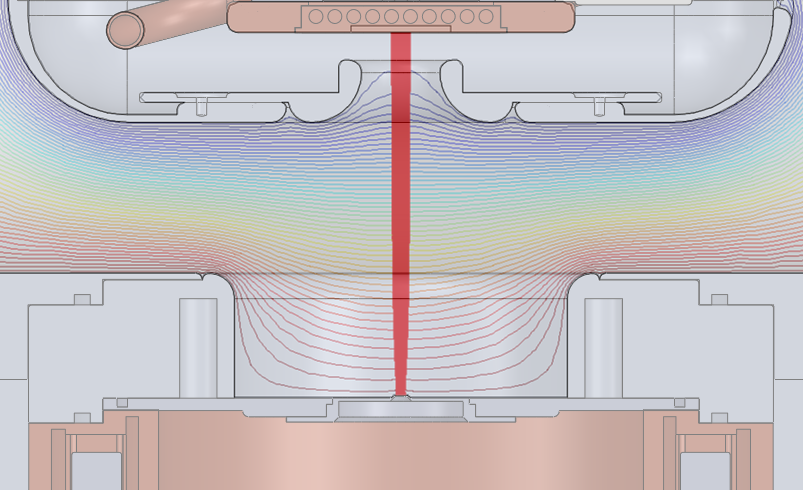
\includegraphics[width=0.55\textwidth]{pics/beam}}
	\hfill
	\subfloat[\label{subfig:beam_in_shroud}]{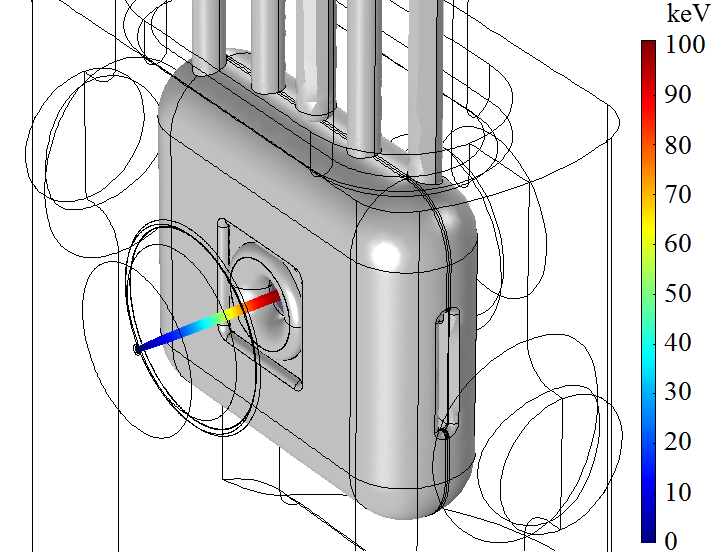
\includegraphics[width=0.445\textwidth]{pics/beam_shroud}}
	\caption{Comsol simulation of electric field and deuteron beam trajectory at 100 kV and 1.4 mA. \DIFaddbeginFL \comment{Make a brief comment to indicate which direction corresponds to the RF source vs the target, to show perspective.  Repeat the comment about the apparent focusing field.}\DIFaddendFL }
	\label{fig:beam_spread}
\end{figure}

The resulting beam spot size and heat deposition on the target are shown in Figure \ref{fig:beam_spot2}. Note that the beam profile in a) is \DIFdelbegin \DIFdel{not uniform }\DIFdelend \DIFaddbegin \DIFadd{non-uniform }\DIFaddend across the target, and  \DIFdelbegin \DIFdel{there is }\DIFdelend localized heating (and neutron production) \DIFaddbegin \DIFadd{is observed }\DIFaddend near the edges. Therefore, a convex-shaped extraction nozzle was designed, whose purpose is to counteract the focusing electric field experienced near the aperture. The nozzle design is shown in Figure \ref{fig:beam_spot2} b) and c). \DIFaddbegin \comment{You mention the convex nozzle, but don;t describe its pitch / the forward and back diameters.  Please elaborate more detail regarding the shape of the nozzle, how you got to that particular design, and provide these numbers in the caption for Fig 9.} \DIFaddend Note the defocusing effect of the nozzle due to the fact that the equipotential lines are slightly convex downstream of the beam path. The beam spot is not only more uniform, but it is also spread throughout a larger area, which reduces the heat load on the target.

\begin{figure}
	\centering
	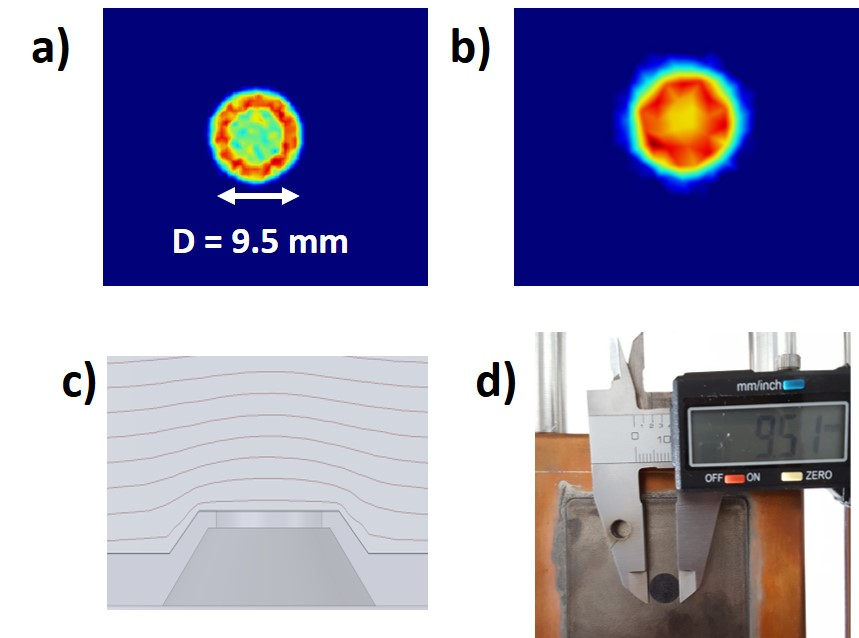
\includegraphics[width=0.7\textwidth]{pics/beam_spot2}
	\caption{Beam spreading by modification of the \DIFaddbeginFL \DIFaddFL{single  0.262 cm diameter }\DIFaddendFL extraction plate \DIFaddbeginFL \DIFaddFL{nozzle}\DIFaddendFL : a) flat extraction, b) \DIFdelbeginFL \DIFdelFL{and }\DIFdelendFL \DIFaddbeginFL \& \DIFaddendFL c) convex extraction, d) burn mark on target.\DIFaddbeginFL \comment{Confirm that this is teh correct diamater in the caption, and describe / label the convex nozzle geometry. }\DIFaddendFL }
	\label{fig:beam_spot2}
\end{figure}

Experimental results show a high degree of consistency with simulations based on the beam spot size (diffuse burn mark measured to be around 10 mm), and the resulting neutron flux distribution, as detailed in Chapter 5. 

\DIFaddbegin \comment{This claim is more appropriate to be included in the validation / section 5.  Consider moving it there, and expand on this.  What does ``high degree of consistency'' mean?  Elaborate and use numbers.}


\DIFaddend \subsection{Multiple-Hole Extraction System}

\DIFaddbegin \comment{You give the multi-hole plate its own subsection, create one for the single-hole plate also.}

\DIFaddend The uniformity of the beam spot and further spread of \DIFdelbegin \DIFdel{impingement area }\DIFdelend \DIFaddbegin \DIFadd{heat load }\DIFaddend can be achieved by \DIFdelbegin \DIFdel{different means }\DIFdelend \DIFaddbegin \DIFadd{alternative means than optimizing a single extraction nozzle}\DIFaddend . For instance, an Einzel lens configuration, \DIFdelbegin \DIFdel{i.e. }\DIFdelend \DIFaddbegin \emph{\DIFadd{i.e.}}\DIFadd{, }\DIFaddend one or more extraction plates located downstream of the beam and biased at different potentials\DIFaddbegin \DIFadd{, }\DIFaddend can give further control of the beam envelope. One of the downsides of such an arrangement is the higher degree of complexity added to the design, which stems from biasing, insulating, and properly installing these plates inside the vacuum chamber. Another option is the use of multiple apertures in the plasma electrode. Figure \ref{fig:CAD_extraction} shows an optimized design of a 19-hole extraction plate arranged in a hexagonal pattern, which was chosen in order to optimize the packing fraction and the uniformity of the beam.

\DIFaddbegin \comment{Why does optimizing packing fraction matter?  Explain.}

\DIFaddend \begin{figure}
	\centering
	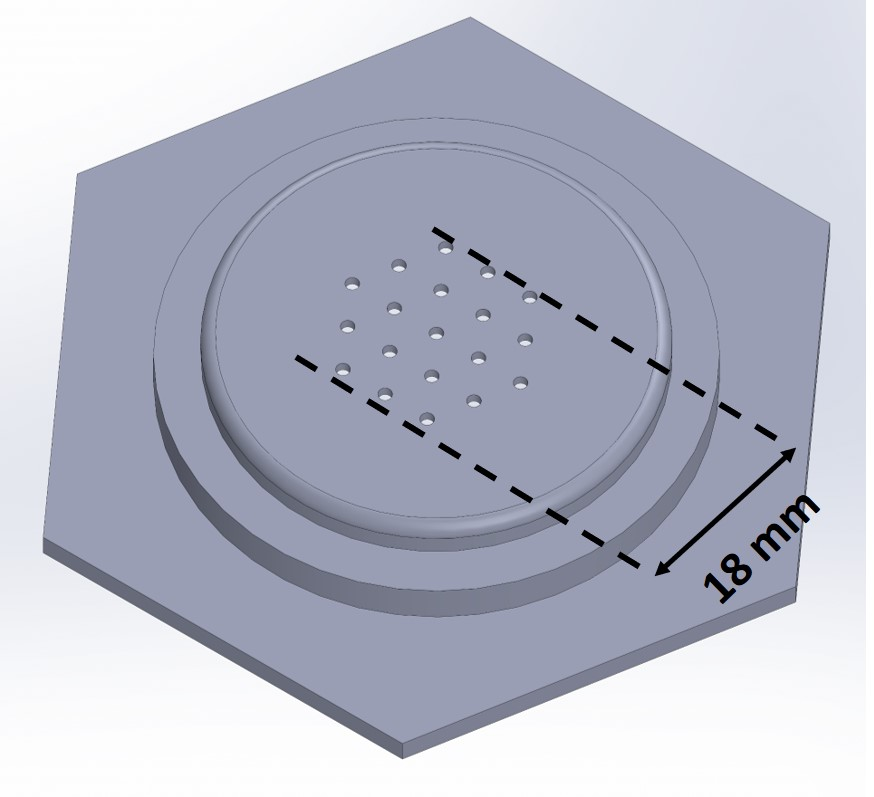
\includegraphics[width=0.5\textwidth]{pics/CAD_plate2}
	\caption{CAD drawing of \DIFdelbeginFL \DIFdelFL{an }\DIFdelendFL \DIFaddbeginFL \DIFaddFL{the }\DIFaddendFL optimized 19-hole extraction plate. \DIFaddbeginFL \comment{Good reference scale.  Mention the diameter of the individual holes.}\DIFaddendFL }
	\label{fig:CAD_extraction}
\end{figure}

In order to approximate the maximum beam current that can be extracted from each individual hole, the \DIFdelbegin \DIFdel{Child Langmuir }\DIFdelend \DIFaddbegin \DIFadd{Child-Langmuir }\DIFaddend law was employed, which sets a limit for the extractable current through an aperture assuming the system is space \DIFdelbegin \DIFdel{charge limited }\DIFdelend \DIFaddbegin \DIFadd{charge-limited }\DIFaddend (enough ions are available in the ion source). This treatment was derived only for beam extraction between parallel plates, but serves as a good approximation for our purposes. \DIFaddbegin \comment{Why? How do you know it to still be applicable?} \DIFaddend Figure \ref{fig:child_lang} shows the maximum theoretical beam current that can be extracted as a function of the aperture diameter for the HFNG geometry at 100 kV. \DIFdelbegin \DIFdel{Because it is in our interest }\DIFdelend \DIFaddbegin \comment{Where does this data coem from? Child-Langmuir law? Explain and provide a citation.} \DIFadd{Because it desirable }\DIFaddend to keep the diameter of the apertures small \DIFaddbegin \comment{Why, if you could get more current extracted?  Elaborate a bit briefly on the tradeoff, and how to find a ``sweet spot''.}\DIFaddend , we chose a diameter of $1\ mm$, through which it is possible to draw a current of \DIFdelbegin \DIFdel{$\approx 0.196\ mA$}\DIFdelend \DIFaddbegin \DIFadd{$\approx 0.196$ mA}\DIFaddend . Therefore, for the 19-hole plate arrangement, it is theoretically possible to draw up to \DIFdelbegin \DIFdel{$3.7\ mA$}\DIFdelend \DIFaddbegin \DIFadd{$3.7$ mA}\DIFaddend , or a total of \DIFdelbegin \DIFdel{$7.4\ mA$ }\DIFdelend \DIFaddbegin \DIFadd{$7.4$ mA }\DIFaddend if both ion sources are used. This current  \DIFdelbegin \DIFdel{value }\DIFdelend is an approximation, but it serves as a conservative input parameter for  \DIFdelbegin \DIFdel{the }\DIFdelend ion beam simulations. In fact, the observed current limit was 3.5 mA, confirming the validity of this approximation. \DIFaddbegin \comment{Nice!}
\DIFaddend 

 \begin{figure}
 	\centering
 	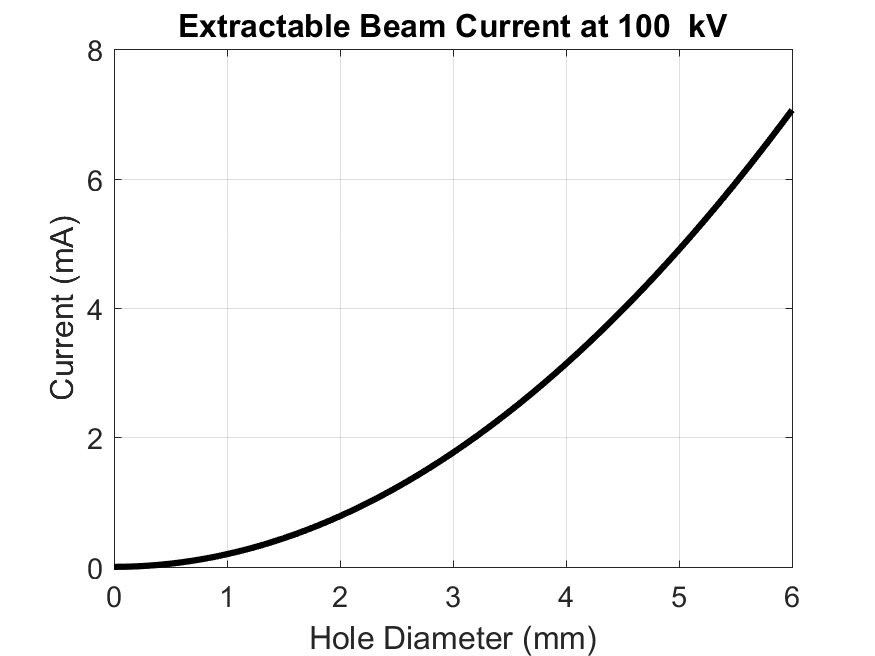
\includegraphics[width=0.7\textwidth]{pics/childLang}
 	\caption{Maximum extractable current according to Child Langmuir law for the HFNG geometry at 100 kV. \DIFaddbeginFL \comment{Provide citation for Child-Langmuir here.}\DIFaddendFL }
 	\label{fig:child_lang}
 \end{figure} 

Simulations show a more uniform beam profile near the center and a larger impingement area, which translates into a lower heat flux than that of a single hole even at higher current values. Beam current can be further increased by adding more holes or by increasing the \DIFdelbegin \DIFdel{size }\DIFdelend \DIFaddbegin \DIFadd{diameter }\DIFaddend of the holes. The increase in current can be limited by the maximum number of holes that can be drilled on the plate or by the increase in chamber pressure due to a larger open area between the ion source and the rest of the vacuum chamber. The latter could \DIFdelbegin \DIFdel{make }\DIFdelend \DIFaddbegin \DIFadd{raise }\DIFaddend the gas pressure too high for optimum operation. \DIFaddbegin \comment{What pressure limit would this be?}
\DIFaddend 

The geometry of the HFNG is such that there exists a focusing electric field at extraction, as shown in Figure \ref{fig:beam_spread}. Therefore, off-centered beamlets experience a focusing force, which depends on their location with respect to the center. For instance, beamlets further away from the center experience a stronger focusing force because the equipotential lines are more concave in that region. Therefore, multiple-extraction hole systems produce a convergent beam envelope. In contrast, a single hole in the center produces a divergent beam envelope, as shown in Figure \ref{fig:single_vs_mult}. The reason for this spread is \DIFdelbegin \DIFdel{somewhat }\DIFdelend \DIFaddbegin \DIFadd{partially }\DIFaddend due to space charge \DIFdelbegin \DIFdel{. However, the main reason is }\DIFdelend \DIFaddbegin \DIFadd{effects, but is primarily due to }\DIFaddend the initial focusing provided by the extraction hole itself, which causes deuterons to cross over and then diverge. This phenomenon is depicted in Figure \ref{fig:cross_over}. \DIFaddbegin \comment{Not sure if Fig 12 shows this clearly or not.} \DIFaddend Essentially, each extracting aperture acts as a non-linear electrostatic lens with spherical aberration (not focused to a point) \cite{Plasma}. 

\DIFaddbegin \comment{This citation appears to be broken in your google drive version.}

\DIFaddend \begin{figure}
	\centering
	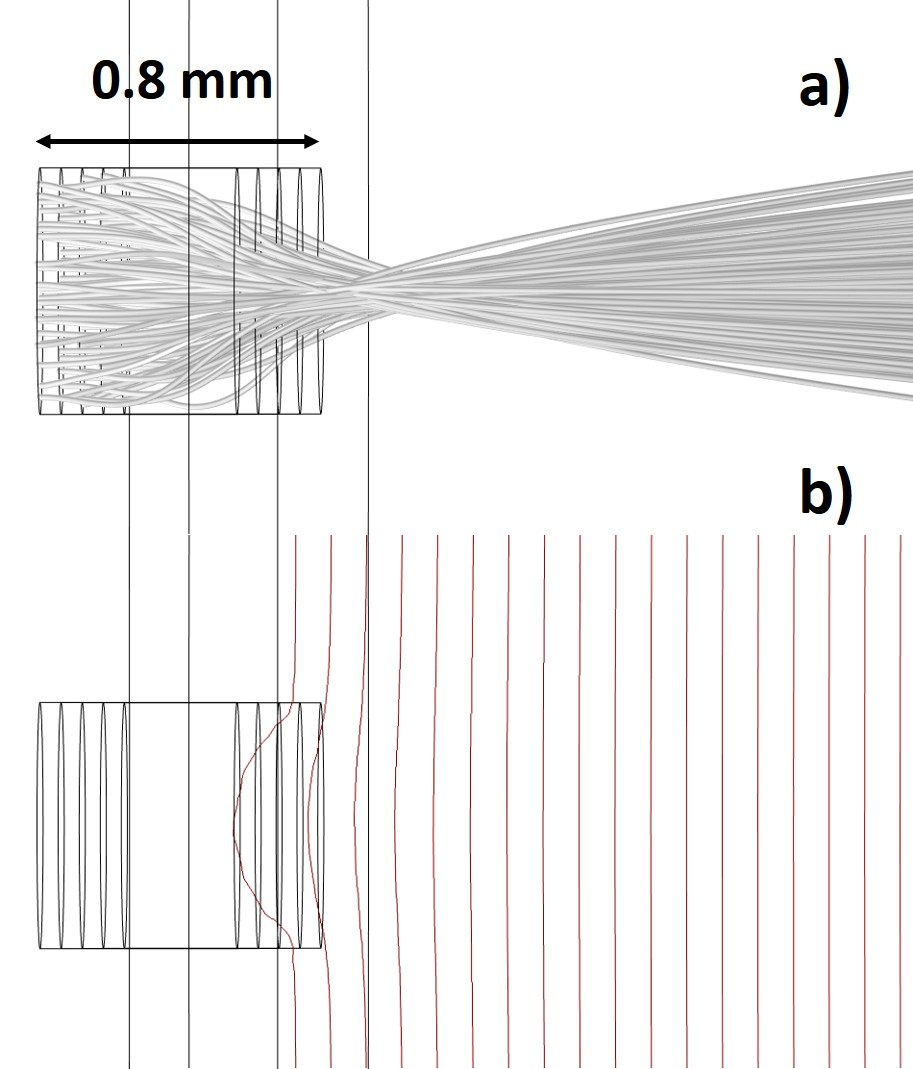
\includegraphics[height=0.6\textwidth]{pics/cross_over_comp}
	\caption{Simulation of deuteron trajectories near extraction. Note the convergent field (b) that provides the initial focusing force that is ultimately responsible for the spreading of the beam. \DIFaddbeginFL \comment{Figure is a bit unclear as to what it actually shows.  Label or describe where extraction, the ion sourecs and the target are, to illustrate the convergence, as its unclear currently.}\DIFaddendFL }
	\label{fig:cross_over}
\end{figure}

\begin{figure}
	\centering
	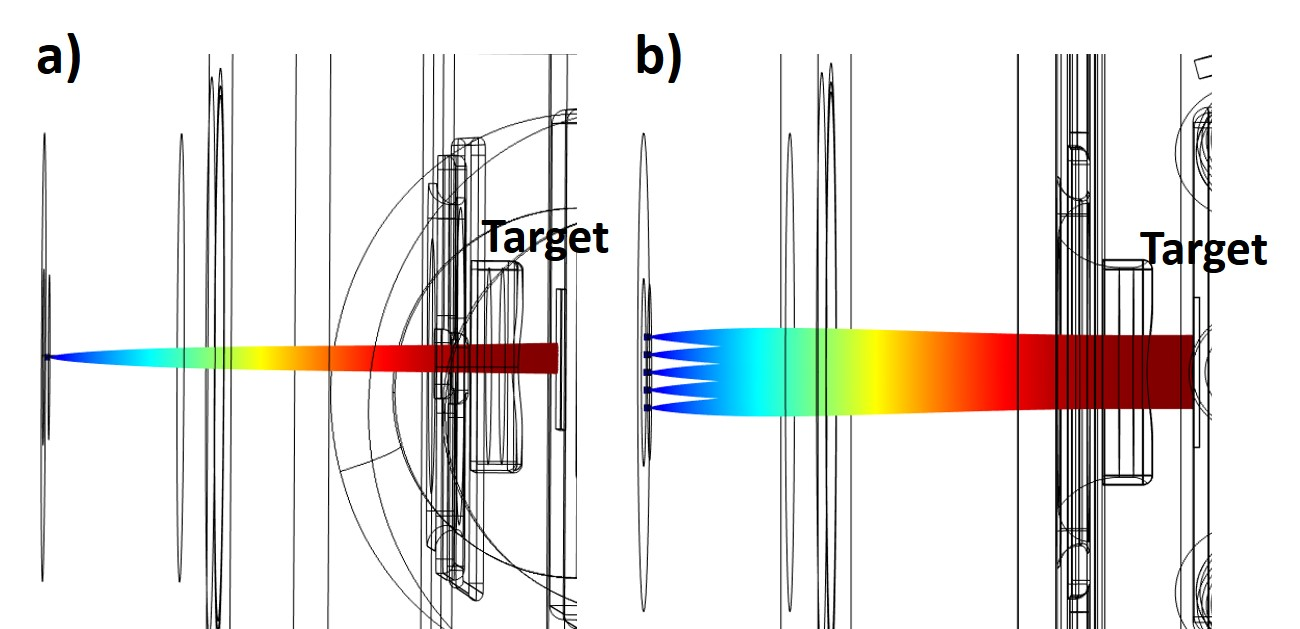
\includegraphics[height=0.5\textwidth]{pics/single_vs_mult2}
	\caption{The beam envelope for a single beam\DIFaddbeginFL \DIFaddFL{, a),  }\DIFaddendFL located at the center is divergent while that of multiple holes\DIFaddbeginFL \DIFaddFL{, b), }\DIFaddendFL is convergent.}
	\label{fig:single_vs_mult}
\end{figure}

\DIFaddbegin \comment{What is this spacer?  This is the first time you mention it, so you need to first descrobe what it is, what it does, dimensions, materials, etc.}

\DIFaddend If there were no spacer, the beamlets would not experience a focusing force and the beam envelope would be divergent, as shown in Figure \ref{fig:spacer_vs_noSpacer}. However, at such a close distance (\DIFdelbegin \DIFdel{$\approx 7\ cm$ }\DIFdelend \DIFaddbegin \DIFadd{$\approx$ 7 cm }\DIFaddend from the target), the individual beamlets would not spread enough and the heat deposition per beamlet would be unacceptable.  

\begin{figure}
	\centering
	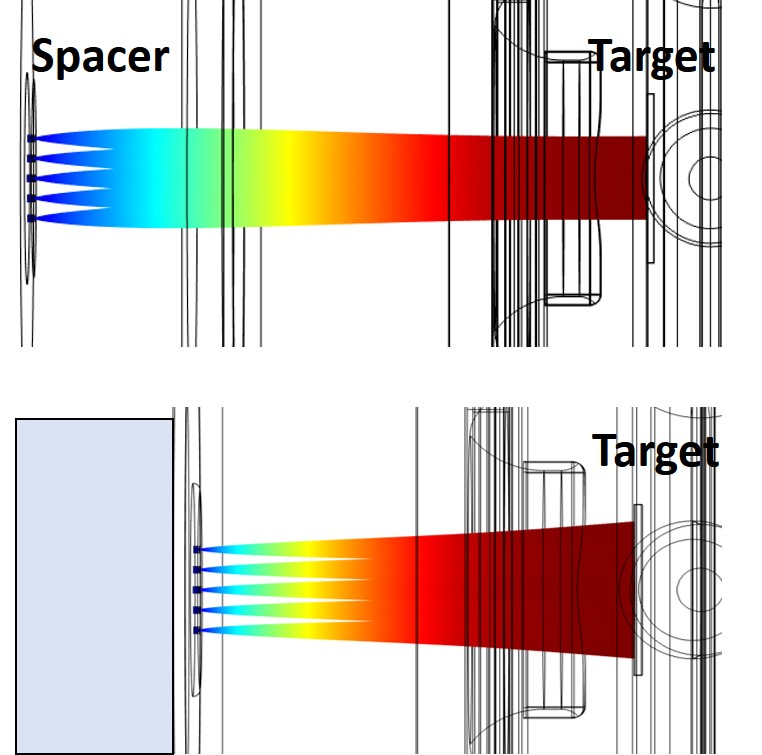
\includegraphics[width=0.5\textwidth]{pics/spacer_vs_noSpacer2}
	\caption{Beam envelope with spacer (top), and without spacer (bottom), showing the effect of the spacer, which gives an additional standoff of 7 cm; the spacer also introduces a focusing field.}
	\label{fig:spacer_vs_noSpacer}
\end{figure}

\DIFaddbegin \comment{Im confused as to what you mean by beamlet center. Please explain before using teh term.  Is it the centroid of the overall beam pattern formed by all the beamlets?  Please elaborate.  Also, pick eitehr ``beamlet center'' or ``beam center'', and be consistent - see Fig 15 x- and y-axis label.} 

\DIFaddend Simulations were performed in order to optimize the hole pattern distribution. The design curve shown in Figure \ref{fig:designC} shows the beamlet center at the target as a function of the beamlet location at the extraction plate. The dashed line shows the hypothetical case in which there is no focusing field and the beamlets are perfectly horizontal.

\DIFaddbegin \comment{What do you mean by perfectly horizontal?  The individual beamlets without a spacer should be divergent, I think.}

\DIFaddend \begin{figure}
	\centering
	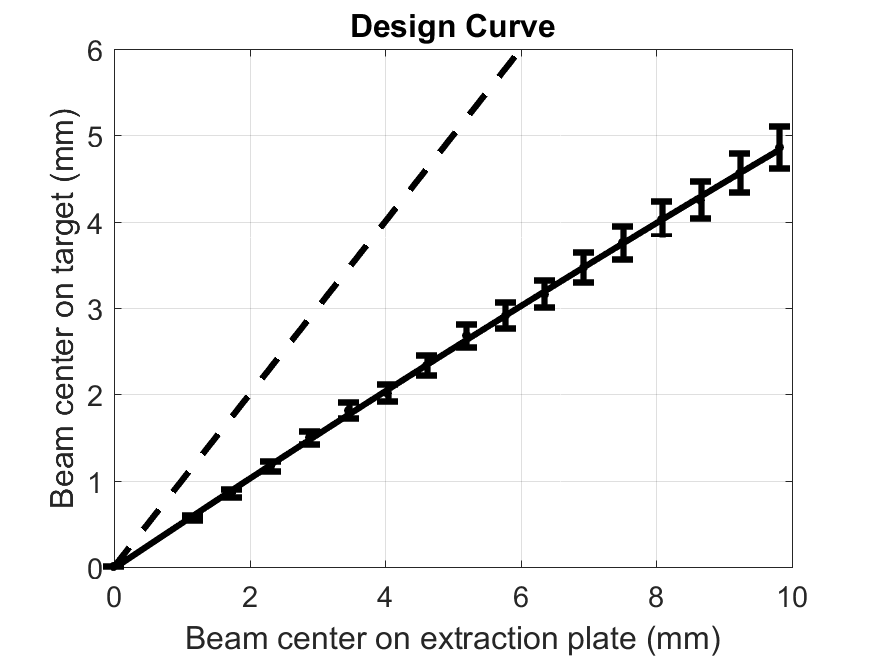
\includegraphics[height=0.5\textwidth]{pics/designC}
	\caption{Design curve used to estimate the center of the individual deuterium beamlets on the target. The dashed curve is for the case with no spacer (linear) and the solid curve for the current configuration. \DIFaddbeginFL \comment{Where does this data come from?  You never describe it anywhere, and it definitely needs to eb added.  Experimental measurement?  Simulation?  If it is simulation, how did you verify / benchmark that the simulations were reliable for the generation of this design curve?  These questions MUST be addressed. Why does teh solid line have uncertainties plotted, but the dashed line does not?  be consistent, and add uncertainties to the dashed line.}\DIFaddendFL }
	\label{fig:designC}
\end{figure}

The optimization process focused on two parameters: reduction of heat flux on the target surface, and uniformity of the heat flux distribution, which translates into a more uniform  \DIFdelbegin \DIFdel{(flat) }\DIFdelend neutron flux distribution at the sample location.

\DIFaddbegin \comment{Why was two rings of nozzles chosen?  Why not 3, or using the number of rings as a design parameter? The motivation behind this decision needs to be made explicitly clear in the text.}

\DIFaddend \begin{figure}
	\centering
	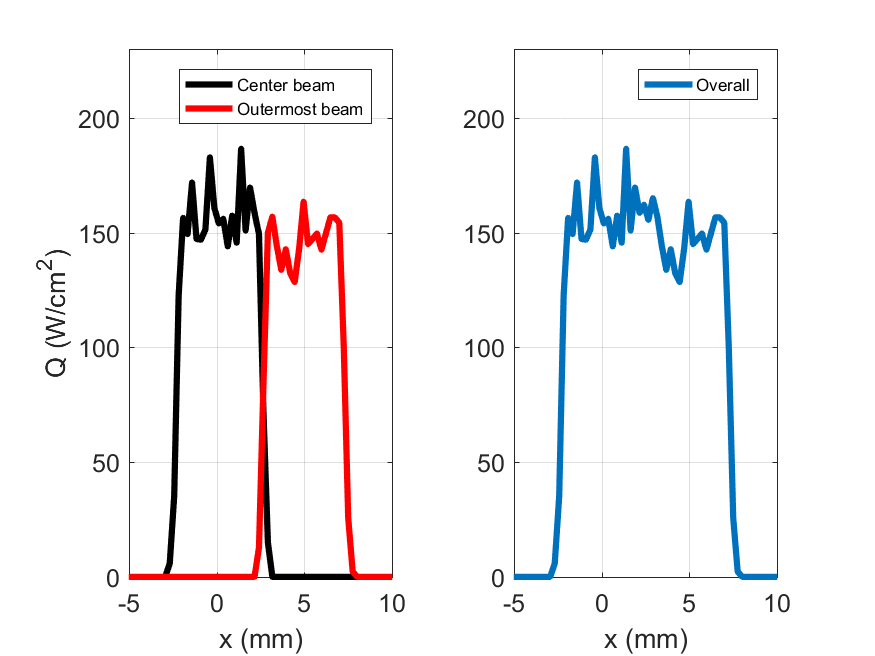
\includegraphics[height=0.5\textwidth]{pics/twoBeams}
	\caption{Comsol simulation results showing the center and outermost beamlets. The latter was placed so as to achieve a flat profile.}
	\label{fig:two_beams}
\end{figure}

\DIFaddbegin \comment{By ``outermost beamlet'', do you mean the beamlet in the outer ring of nozzles?  Please make this more clear.}

\DIFaddend Figure \ref{fig:two_beams} shows the 2D beam profiles of the center beamlet and the outermost beamlet. The latter was placed 9.8 mm from the center in order to achieve a flat beam profile on the target. 
\DIFaddbegin \comment{Is this distance a center-to-center distance, or edge-to-edge? Is it a gap distance, or a pitch? Please make clear.}
\comment{Also, you show this figure, but don't comment on it.  You need to provide some commentary as to the significance of this figure, and what it tells you.}
\DIFaddend The intermediate hole was placed in such a way that its corresponding beamlet would hit the target exactly midway between the other two. This location was calculated (from the design curve) to be 5.1 mm from the center. \DIFaddbegin \comment{Again, specify center-to-center or edge-to-edge.} \DIFaddend The resulting heat flux distribution is shown Figure \ref{fig:heat maps} (right). Note that evenly spaced extraction apertures result in a non-uniform distribution due to the uneven focusing effect explained previously. A design leading to an unacceptable heat profile is shown in Figure \ref{fig:heat maps} (left). 

\DIFaddbegin \comment{This paragraph needs a lot of work and clarification.  You say that the optimized design intermediate beamlets would hit the target exactly midway between the other two, but then turn around and say that evenly spaced extraction apertures result in a non-uniform distribution.  These two statements seem to contradict, so you need to further explain and reconcile them. Also, throughout this work (I've brought it a up a few times now), you keep referencing unacceptable heat loads, or critical failure heat loads, but you have yet to specify a number for this value.  Please give a ballpark number, and stick to it throughout. You also give no information about the pith and nozzle diameter used for it, so the reader has no information about how sensitive the nozzle layout is to heat load, since there is a significant difference seen in the two heat flux maps. This sense of sensitivity needs to be communicated, to show how close or far apart these two designs are in phase space.  Please rework all of this extensively.}

\DIFaddend \begin{figure}
	\centering
	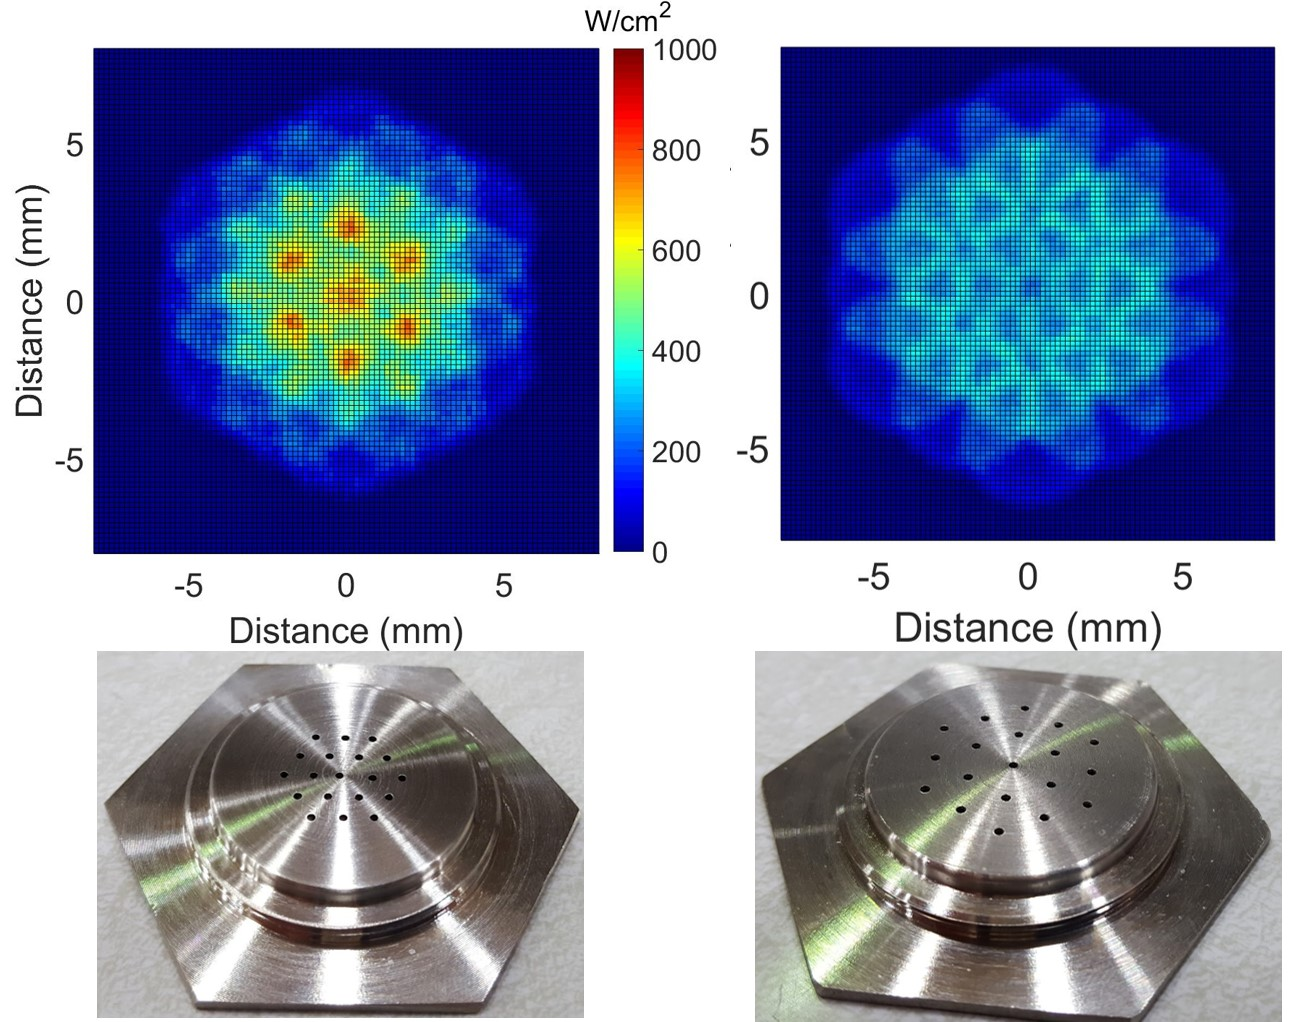
\includegraphics[height=0.6\textwidth]{pics/comparisonHeatMaps_plates2}
	\caption{Power density on the target for a non-optimized design (left) and a design optimized according to the design curve shown in Figure \ref{fig:designC}. \DIFaddbeginFL \comment{See previous comment.  You need to give soem basic info (nozzle pitch and diameter), and comment on the reduced heat flux, removal of hot spots, spread of heat flux over larger area, more uniform heat flux, etc..}\DIFaddendFL }
	\label{fig:heat maps}
\end{figure}

Note that even though the spacing between the holes is larger on the optimized extraction plate design ($d \approx 2 \ cm$), the resulting beam profile on the target is \DIFdelbegin \DIFdel{similar }\DIFdelend \DIFaddbegin \DIFadd{comparable }\DIFaddend in size as the non-optimized design ($d\approx 1.1 \ cm$), but with a higher degree of uniformity and reduced heat flux. Experimental tests validate these simulations, as shown in the experimental validation section.

\DIFaddbegin \comment{Good.  Consider adding a brief comment of the \% difference in beam profile size, as well as a metric to describe the difference in uniformity between the two.}

\DIFaddend \subsection{Heat Transfer Analysis}

The heat flux distribution on the target surface was modeled in \DIFdelbegin \DIFdel{Comsol using the }\DIFdelend \DIFaddbegin \DIFadd{COMSOL using its }\DIFaddend heat transfer in solids module coupled with the turbulent flow module. \DIFaddbegin \comment{What about the (admittedly very low pressure) residual gas?  Does this heat TX model account for passive convection to the residual gas?  This needs to be commented on.} \DIFaddend Further details about the \DIFaddbegin \DIFadd{target's }\DIFaddend heat transfer analysis \DIFdelbegin \DIFdel{on the target can }\DIFdelend \DIFaddbegin \DIFadd{may }\DIFaddend be found in \cite{CoryThesis}. Figure \ref{fig:temp_comsol} shows the temperature distribution on the surface of the target for three different beam profiles: single hole, non-optimized multiple-hole, and optimized multiple-hole extraction plate. \DIFdelbegin \DIFdel{Note that the three of them show maximum temperature values }\DIFdelend \DIFaddbegin \comment{You should reiterate the design specs of each here:  nozzle(s) diameter, and pitch.} \DIFadd{Note that all plate designs show a maximum temperature }\DIFaddend below the degassing temperature of hydrogen in titanium ($\approx 230\ ^{\circ}C)$ \DIFaddbegin \comment{You need to provide a citation for this value!}\DIFaddend . However, the simulations do not account for the inter-metallic phases between the copper and the titanium, or the bonding process itself. Experimentally, it was found that the neutron yield is lower in the case of diffusion bonding compared to the explosion bonded material. This \DIFdelbegin \DIFdel{might }\DIFdelend \DIFaddbegin \DIFadd{would seem to }\DIFaddend indicate that the latter has better heat transfer properties\DIFdelbegin \DIFdel{. Moreover}\DIFdelend \DIFaddbegin \DIFadd{, but XXXXXX. }\comment{Briefly comment again on why better heat TX improves neutron yield, and also provide another possible explanation for the differenec between the two bonding methods.} \DIFadd{Additionally}\DIFaddend , variations in  \DIFdelbegin \DIFdel{the titanium thickness an }\DIFdelend \DIFaddbegin \DIFadd{titanium thickness and the }\DIFaddend purity of the metal \DIFdelbegin \DIFdel{can also }\DIFdelend affect the neutron yield \DIFdelbegin \DIFdel{. The thinner the titanium layer, the better  the }\DIFdelend \DIFaddbegin \DIFadd{-  thinner titanium layers have better  }\DIFaddend heat transfer properties \DIFdelbegin \DIFdel{of }\DIFdelend \DIFaddbegin \DIFadd{in }\DIFaddend the target. \DIFaddbegin \comment{Why is this?  Explain and provide sources.  Also, give rough figures of merit, e. g., a reduction in titanium thickness of 5\% improves heat transfer by 10\%.  Find actual numbers and insert them, and provide a counterargument for going too thin`- insufficient thickness for titanium to implant, I would assume.  You make a claim that thinner targets are better, so you need to back that up with ballpark numbers to illustrate how strong of an effect it is.} \DIFaddend The disadvantage of having a very thin \DIFaddbegin \DIFadd{(less than XXXX mm) }\DIFaddend titanium layer is that the target has a shorter lifetime due to ion sputtering.  \DIFaddbegin \comment{Fill in values, provide approximate target lifetime for this minimum thickness.  Wouldn't an incredibly thin target also be insufficient to have Ti implant, dramatically lowering neutron yield, since titanium is far better of a getter for hydrogen than copper?}
\DIFaddend 


\begin{figure}
	\centering
	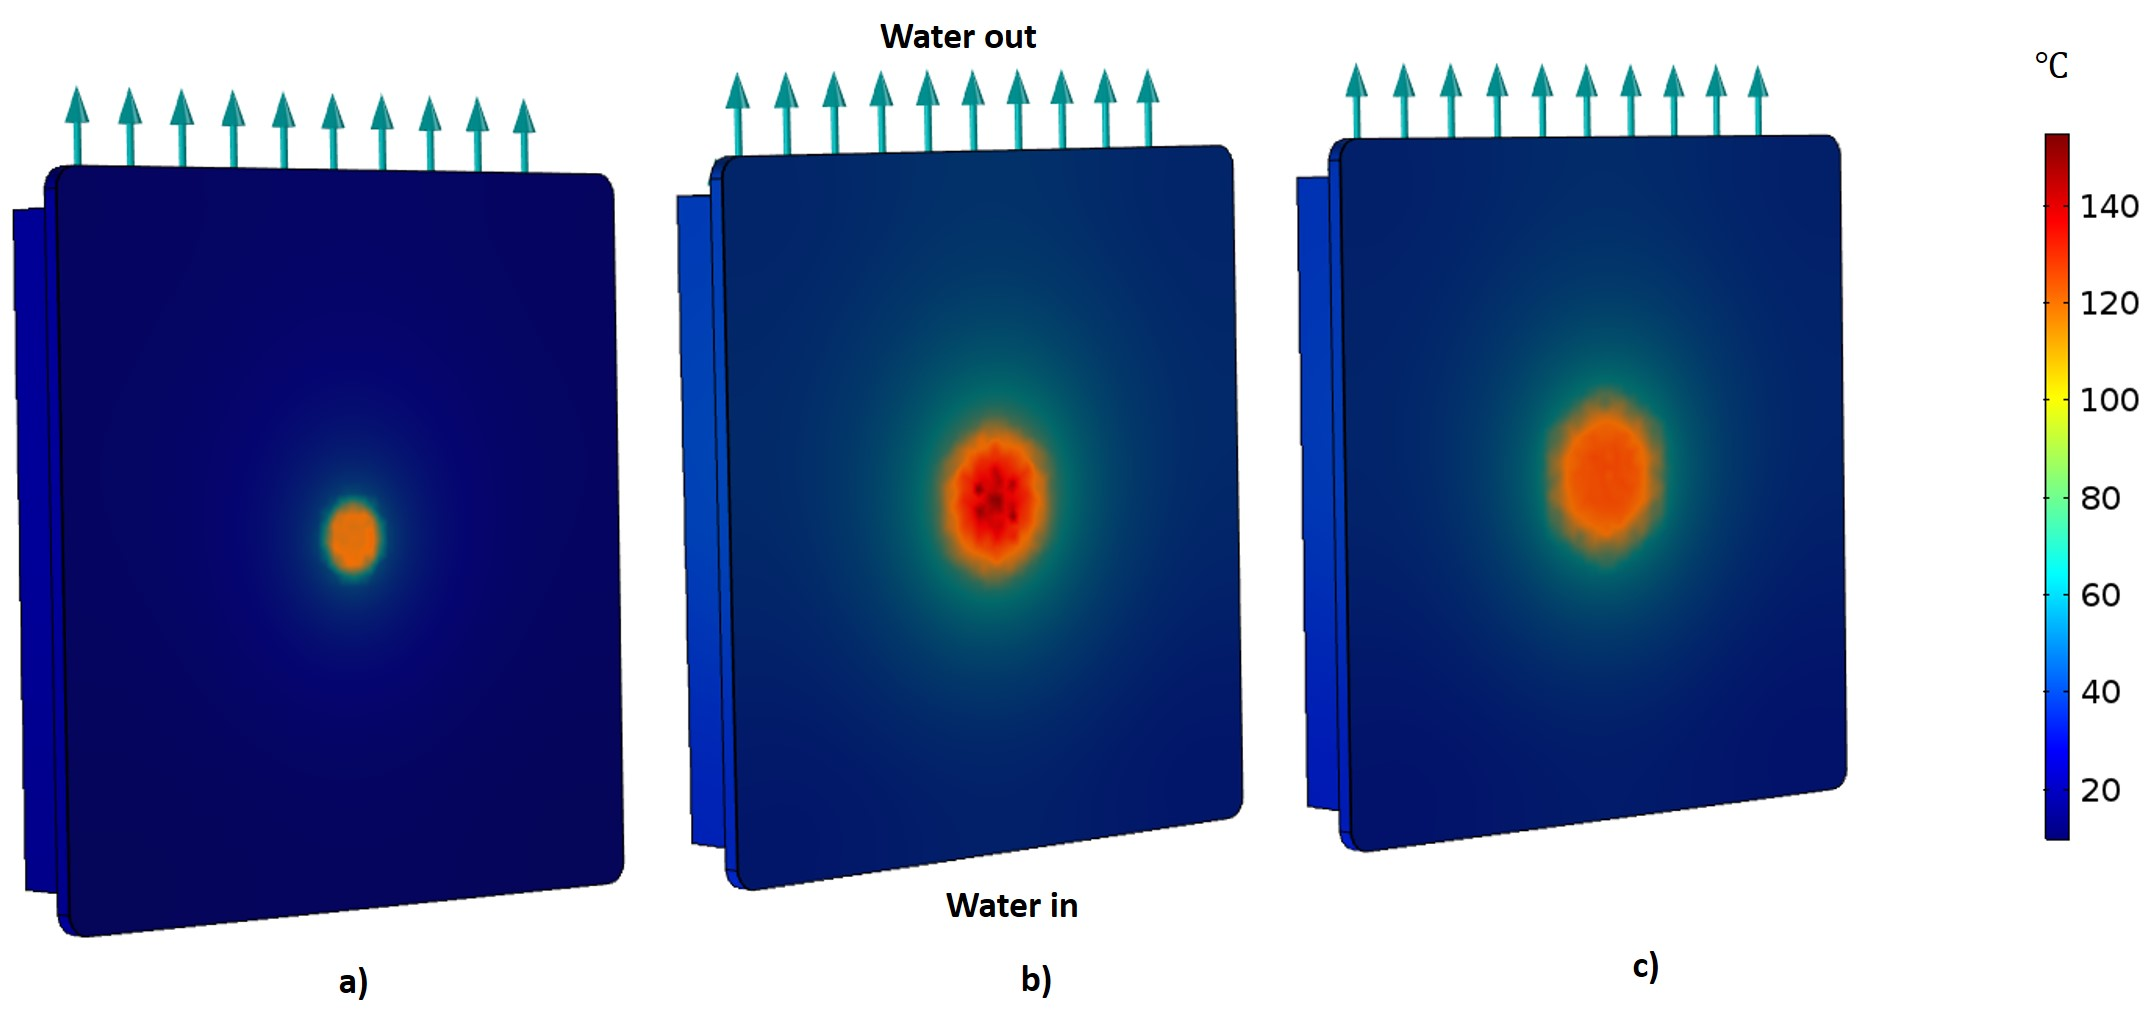
\includegraphics[height=0.5\textwidth]{pics/temp_profiles2}
	\caption{Temperature maps on the target for different extraction plates a) single-hole b) multiple-hole, non-optimized, c) Multiple-hole optimized. Maximum temperature values are $104^{\circ}C$,  $155^{\circ}C$,  \DIFdelbeginFL \DIFdelFL{$114^{\circ}C$}\DIFdelendFL \DIFaddbeginFL \DIFaddFL{$114^{\circ}$C}\DIFaddendFL , respectively\DIFaddbeginFL \DIFaddFL{.  }\comment{Very good.}\DIFaddendFL }
	\label{fig:temp_comsol}
\end{figure}

\begin{figure}
	\centering
	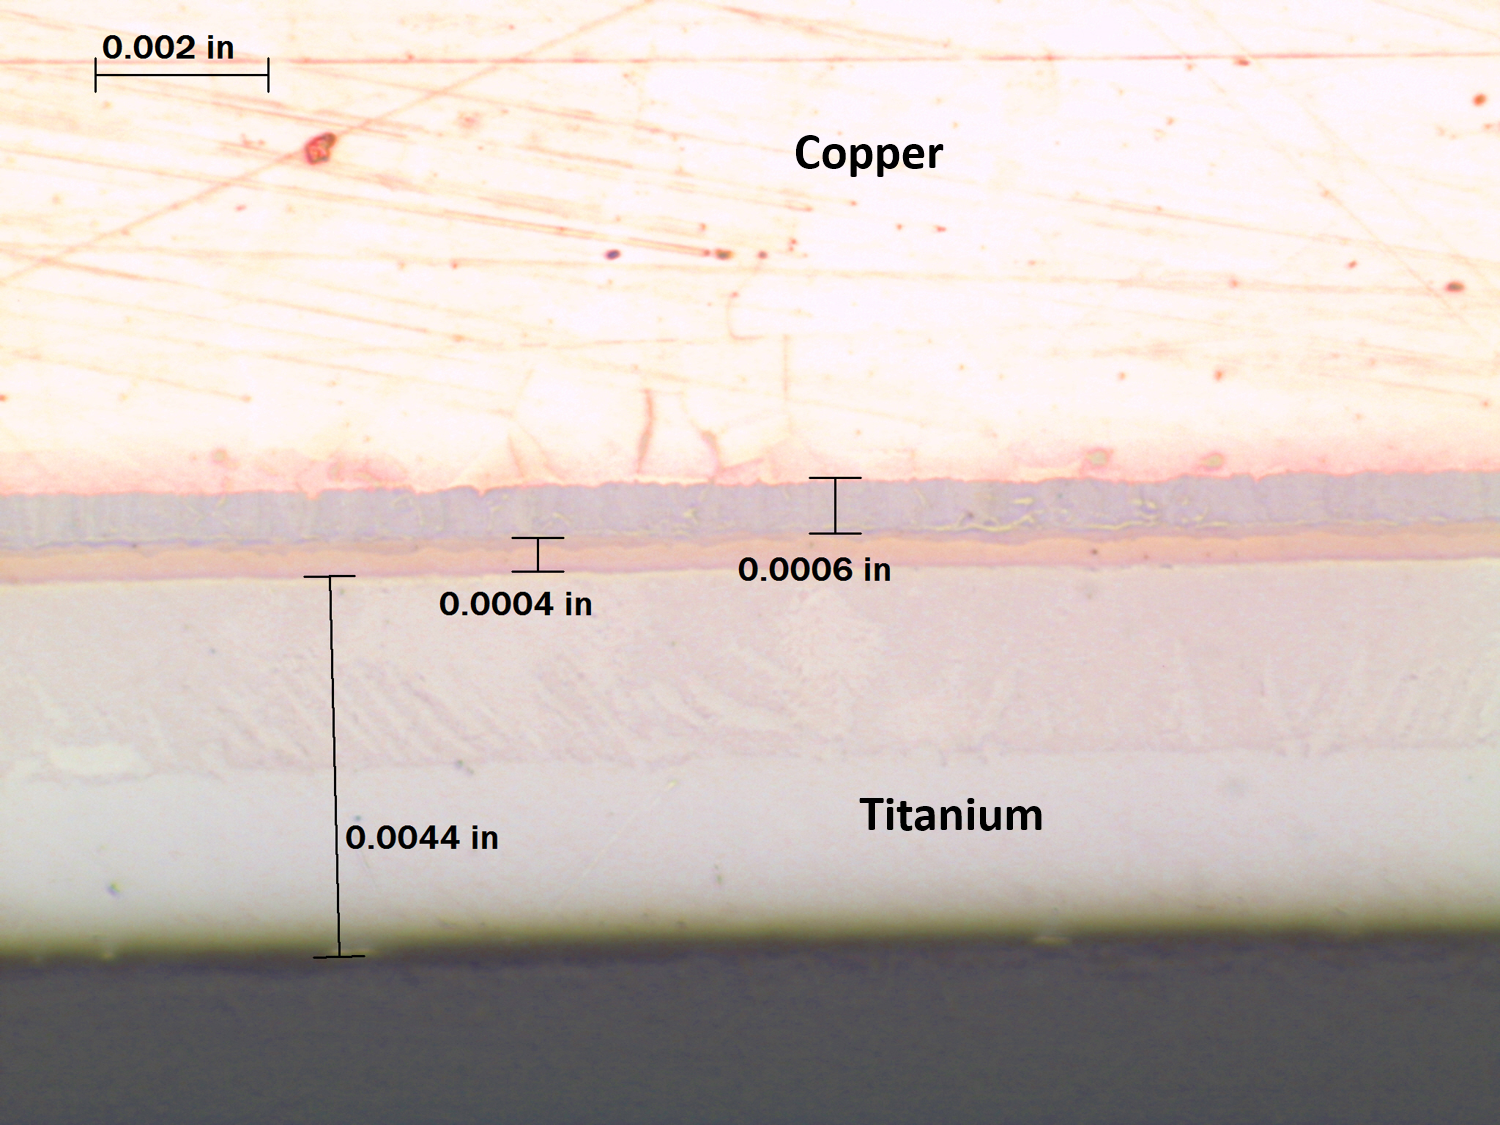
\includegraphics[height=0.5\textwidth]{pics/TiCu2}
	\caption{Metallographic \DIFdelbeginFL \DIFdelFL{test on }\DIFdelendFL \DIFaddbeginFL \DIFaddFL{cross-section of }\DIFaddendFL the HFNG target\DIFaddbeginFL \DIFaddFL{, clearly }\DIFaddendFL showing the \DIFaddbeginFL \DIFaddFL{Cu$_\text{x}$Ti$_\text{y}$ }\DIFaddendFL intermetallic phases between copper and titanium. \DIFaddbeginFL \comment{You use $\micro$m in the text as a length scale, but inches here.  Pick one and be consistent for both.  I would go with $\micro$m.}\DIFaddendFL }
	\label{fig:TiCu}
\end{figure}

Figure \ref{fig:TiCu} shows a metallographic  \DIFdelbegin \DIFdel{test }\DIFdelend \DIFaddbegin \DIFadd{cross-section }\DIFaddend of the diffusion bonded target. Note that there is a region of about 25 \DIFdelbegin \DIFdel{$\mu m$ }\DIFdelend \DIFaddbegin \DIFadd{$\micro$m }\DIFaddend in the copper-titanium interface with two visible phases (\DIFdelbegin \DIFdel{CuTi }\DIFdelend \DIFaddbegin \DIFadd{Cu$_\text{x}$Ti$_\text{y}$ }\DIFaddend intermetallics), which is difficult to include in the simulations and their effect on the heat transfer is unknown. \DIFaddbegin \comment{This seems like a MAJOR red flag for a reviewer. You can actually fairly easily estimate the relative Cu/Ti composition, using an SEM / electron backscatter spectrometer, to gauge the relative abundance of Ti/Cu in each of the phases. Hosemann has such a capability, and we had to use it in 120.  I agree that the impact of this layer should be minor, but this seems to me like something that absolutely could not be published without addressing. I would see if you can use Hosemann's SEM (or have one of his grad students do it) to get this ratio in each phase, and incorporate it into you modeling.  This seems absolutely necessary.} \DIFaddend However, the titanium thickness in the simulated model can be increased by that amount in order to remain conservative. \DIFaddbegin \comment{Not necessarily conservative, as you;ve already noted before that its thermal and deuteride forming properties are significantly different than copper.  The impact should be minor, but we need to address this.} \DIFaddend Experimentally, it was determined that there is some overheating of the target in the case of the non-optimized extraction plate. This was evidenced by the initial increase in neutron dose rate rapidly followed by a decrease \DIFdelbegin \DIFdel{rate. }\DIFdelend \DIFaddbegin \DIFadd{in dose rate. }\comment{This does not follow.  How does overhetaing lead to increased neutron yield, then reduced yield?  please explain in text.} \DIFaddend The neutron yield in this case was similar to that of the single-hole extraction plate. However, the optimized geometry \DIFaddbegin \comment{single-hole or multi-hole?  Please clarify.} \DIFaddend allows for an increase in neutron yield by a factor of $\approx 2.5$, which is expected from Equation \ref{eq:yield}.  

\DIFaddbegin \comment{Your last sentence here doesn't make sense.  What parameter in Eqn 3 is being increased by the optimized design causing this factor of 2.5 increase in neutron yield?  Reword the sentence and be more specific, your logic doesn't follow.}

	
\DIFaddend \section{Experimental Validation of the Neutron Flux and Deuteron Beam Profile}	

The neutron flux was experimentally determined \DIFdelbegin \DIFdel{by neutron activation analysis }\DIFdelend \DIFaddbegin \DIFadd{through neutron irradiation }\comment{Neutron activtaion analysis typically refers more to (n,$\gamma$) analysis of abundance in a sample, and doesn't really precisely apply here.} \DIFaddend of nine natural indium foils arranged in a $3\times3$ array at the sample holder location\DIFaddbegin \DIFadd{, as }\DIFaddend shown in Figure \ref{fig:flux_map}. \DIFaddbegin \comment{Do you have a picture of the 3x3 sample holder? I think it would eb useful to include here, too.} \DIFaddend Indium is a soft metal \DIFdelbegin \DIFdel{that }\DIFdelend \DIFaddbegin \DIFadd{which }\DIFaddend can be easily cut \DIFdelbegin \DIFdel{or machined to the desired size and shape. The foils were cut in the form of thin disks of about }\DIFdelend \DIFaddbegin \DIFadd{into foils approximately }\DIFaddend 0.9 cm in diameter \DIFdelbegin \DIFdel{. The isotope In-115 has a long lived ($t_{1/2}=4.486\ h$) isomer that }\DIFdelend \DIFaddbegin \DIFadd{and XXX mm thick  }\comment{Fill in thickness values.}\DIFadd{. The naturally-occurring isotope $^{115}$In has a long-lived ($^{115\text{m}}$In t$_{1/2}=4.486 \pm 0.004$ h, IT=95.0 $\pm$ 0.7 }\% \DIFadd{to $^{115}$In \mbox{%DIFAUXCMD
\cite{Blachot2012}
}%DIFAUXCMD
) }\comment{Always cite the more recent NDS evaluation when quoting a half-life.  Use \url{http://linkinghub.elsevier.com/retrieve/pii/S0090375212000683} here.} \DIFadd{isomer which }\DIFaddend decays by the emission of a \DIFdelbegin \DIFdel{336 }\DIFdelend \DIFaddbegin \DIFadd{336.241 }\DIFaddend keV gamma ray to \DIFdelbegin \DIFdel{the }\DIFdelend \DIFaddbegin \DIFadd{its }\DIFaddend ground state; this \DIFdelbegin \DIFdel{metastable state }\DIFdelend \DIFaddbegin \DIFadd{isomer }\DIFaddend is populated by the \DIFdelbegin \DIFdel{reaction
}%DIFDELCMD < 

%DIFDELCMD < %%%
\begin{displaymath}\DIFdel{ \nonumber
^{115}In(n,n')^{115m}In
\label{eqn:In115m}
}\end{displaymath}
%DIFAUXCMD
%DIFDELCMD < 

%DIFDELCMD < %%%
\DIFdelend \DIFaddbegin \DIFadd{inelastic scattering reaction $^{115}$In(n,n')$^{115\text{m}}$In.
%DIF >  \begin{equation} \nonumber
%DIF >  ^{115}In(n,n')^{115m}In
%DIF >  \label{eqn:In115m}
%DIF >  \end{equation}
}\DIFaddend The nine indium foil arrangement allows for  \DIFdelbegin \DIFdel{precise }\DIFdelend \DIFaddbegin \comment{With only 3 pixels in each axis, we can't really call it ``precise.''} \DIFaddend determination of the beam spot location with respect to the \DIFdelbegin \DIFdel{samples to be irradiated . Hence}\DIFdelend \DIFaddbegin \DIFadd{9 irradiated samples. Through the combination of MCNP modeling of neutron transport and  decay spectroscopy of the activated indium foils}\DIFaddend , the energy window \DIFdelbegin \DIFdel{can be well characterized for any given experiment}\DIFdelend \DIFaddbegin \DIFadd{and flux distribution subtended by each of the foils can be well-characterized for a given target configuration}\DIFaddend . Further details on the flux \DIFdelbegin \DIFdel{measurements }\DIFdelend \DIFaddbegin \DIFadd{characterization }\DIFaddend can be found in \DIFaddbegin \DIFadd{the recent work of A.S. Voyles }\emph{\DIFadd{et al.}} \DIFaddend \cite{np_paper}.  

The flux map for an \DIFdelbegin \DIFdel{experiment }\DIFdelend \DIFaddbegin \DIFadd{irradiation }\DIFaddend carried out at 100 kV and 1.4 mA is shown in Figure\ref{fig:flux_map}. Based on this \DIFdelbegin \DIFdel{experiment}\DIFdelend \DIFaddbegin \DIFadd{beam profile, simulated using XXXXXXXX}\DIFaddend , it was determined that the \DIFdelbegin \DIFdel{center foil }\DIFdelend \DIFaddbegin \DIFadd{central foil in this 3 x 3 array }\DIFaddend was located 0.5 mm above and 3.7 mm to the right\DIFaddbegin \DIFadd{, }\DIFaddend relative to the center of \DIFdelbegin \DIFdel{where }\DIFdelend the deuterium ion beam\DIFdelbegin \DIFdel{strikes the surface of the target.}\DIFdelend \DIFaddbegin \DIFadd{.. 
}

\comment{Describe source of data for beam profile/}
\DIFaddend 

\begin{figure}
	\centering
		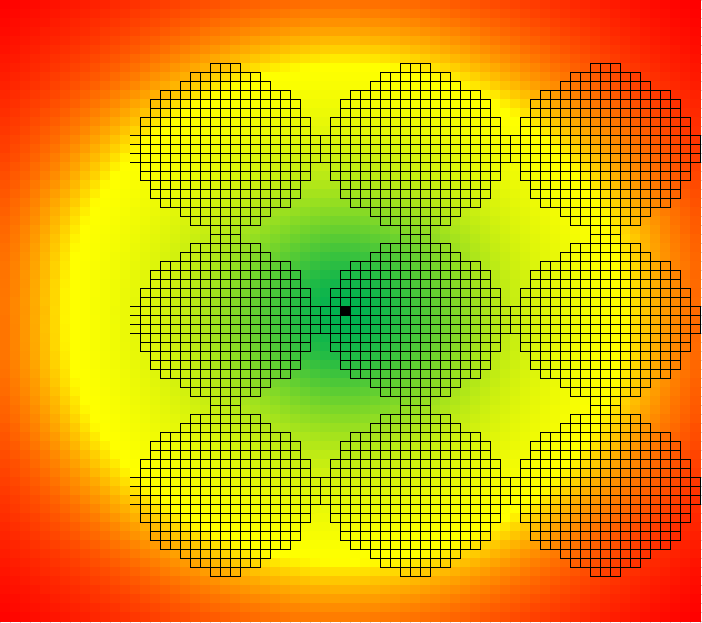
\includegraphics[width=0.9\textwidth]{pics/flux_map}
	\caption{\DIFdelbeginFL \DIFdelFL{Foil }\DIFdelendFL \DIFaddbeginFL \DIFaddFL{3 x 3  indium foil }\DIFaddendFL locations \DIFdelbeginFL \DIFdelFL{compared to }\DIFdelendFL \DIFaddbeginFL \DIFaddFL{superimposed over }\DIFaddendFL the beam center \DIFaddbeginFL \DIFaddFL{for XXXXX extraction plate; beam profile data calculated using XXXXXXX}\DIFaddendFL . \DIFaddbeginFL \DIFaddFL{The beam center is clearly vertically centered on the middle of the loaded samples, with a slight asymmetry of the neutron flux in the horizontal direction. }\comment{Is teh black dot the location of the single nozzle? If so, comment on this in the caption.  You need a length/distance scale included for this figure, either one of the foils, or for the width of the whole thing.  Why are the foils drawn as pixel maps?  The activation of each foil is an integral measurement, so we can't really subdivide them.  Remove the internal grid markers.  Where does the data for the beam profile come from?  You need to describe that in both the text, and briefly comment in the caption.  The beam profile clearly has a color scale, you need to include that scale in this figure.}\DIFaddendFL }
	\label{fig:flux_map}
\end{figure}   

The multiple-hole extraction system was also \DIFdelbegin \DIFdel{tested and the results were compared to simulations. }\DIFdelend \DIFaddbegin \DIFadd{validated in a similar fashion. }\comment{You had mentioned that it was also compared to simulations.  Where is teh figure (comparable to Fig 20) illustrating the results of the simulations?  You can't just say that you compared your experimental results to simulations without showing proof.} \DIFaddend Figure \ref{fig:chamfered} shows the non-optimized beam spot on the target. \DIFaddbegin \comment{Briefly mention the nozzle diameter and pitch info again here.} \DIFaddend Note that the hot spots (darker) can be observed exactly where simulations show they would be, as shown in Figure \ref{fig:heat maps} (a).  \DIFaddbegin \comment{You should remove the referenec to Fig 17a here, and instead put another figure here (similar to Fig 20), overlaying the location of the multi nozzles over your calculated heat map and the 3x3 foils, like Fig 20.  This would be far more useful, and would condense all this information nicely, rather than forcing the reader to flip back and forth.} \DIFaddend The irregular pattern is due to an attempt to remedy the situation by chamfering a few holes on the vacuum side to about $60^{\circ}$ in order to achieve an arrangement closer to a pierce-like \DIFaddbegin \comment{What does this mean?  the description of pierce-like is too vague to determine what you mean to say.} \DIFaddend angle geometry, and thus reducing the heat flux by spreading the individual beamlets. However,  \DIFdelbegin \DIFdel{the chamfering  also enlarged }\DIFdelend \DIFaddbegin \DIFadd{chamfering  enlarges }\DIFaddend the holes, leading to increased current in the \DIFaddbegin \DIFadd{modified }\DIFaddend beamlets, counteracting the intended reduction \DIFaddbegin \DIFadd{and instead increasing the size of hot spots}\DIFaddend .

\begin{figure}
	\centering
	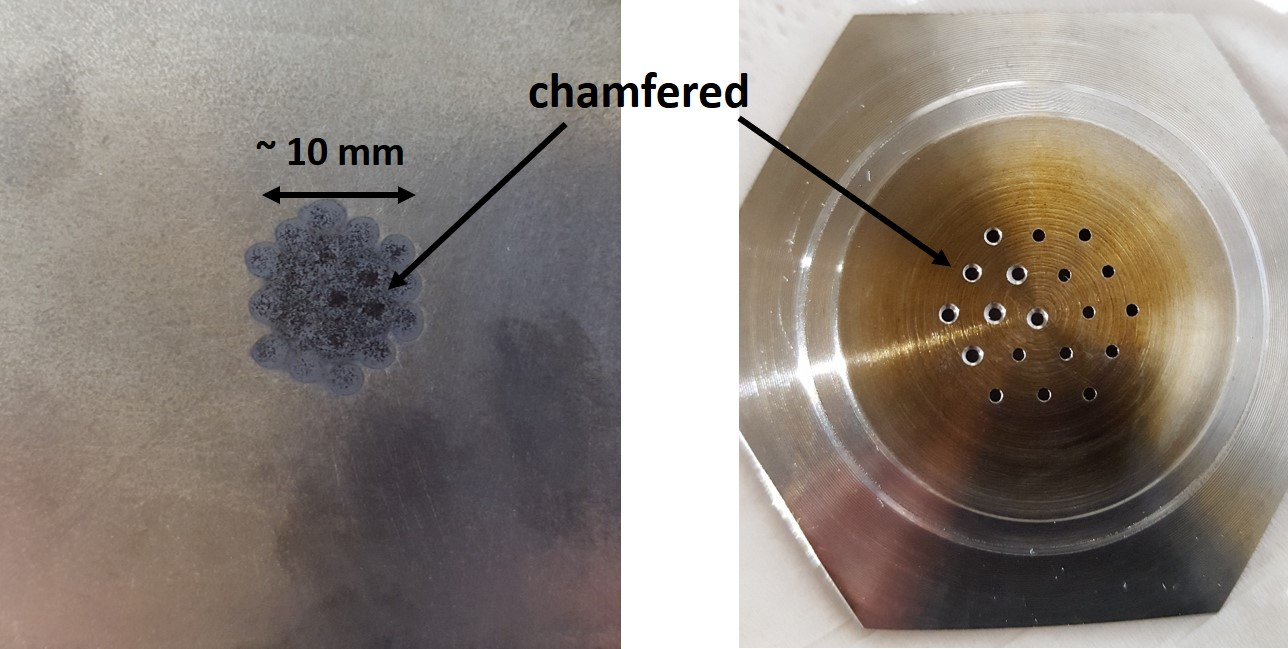
\includegraphics[width=0.9\textwidth]{pics/chamfered}
	\caption{Non-optimized design with a few chamfered holes and the corresponding beam spot. \DIFaddbeginFL \DIFaddFL{The hot spots formed by increased heat load are clearly visible as darkened spots.  The chamfered nozzles appear to increase the intensity and size of these hot spots, rather than making the heat load more uniform.}\DIFaddendFL }
	\label{fig:chamfered}
\end{figure}  

Figure \ref{fig:optimized_notChamfered} shows the beam spot of the optimized extraction plate. \DIFaddbegin \comment{Briefly mention the nozzle diameter and pitch info again here.} \DIFaddend Note that the beam size is accurately predicted by simulations, and it is similar in size \DIFdelbegin \DIFdel{as }\DIFdelend \DIFaddbegin \DIFadd{to }\DIFaddend the non-optimized plate.  \DIFaddbegin \comment{Same issue again. You refer to simulations accurately predicting experiments, but don't show any proof here.  Make a figure here, like for the non-optimized design, (similar to Fig 20), overlaying the location of the multi nozzles over your calculated heat map and the 3x3 foils, like Fig 20.  } \DIFaddend The neutron flux at the central location was increased by a factor of 3.5 with such an arrangement.  \DIFaddbegin \comment{Where does this number come from?  You can't just pull it out of the air, you must show how you calculated / measured it.}
\DIFaddend 

\begin{figure}
	\centering
	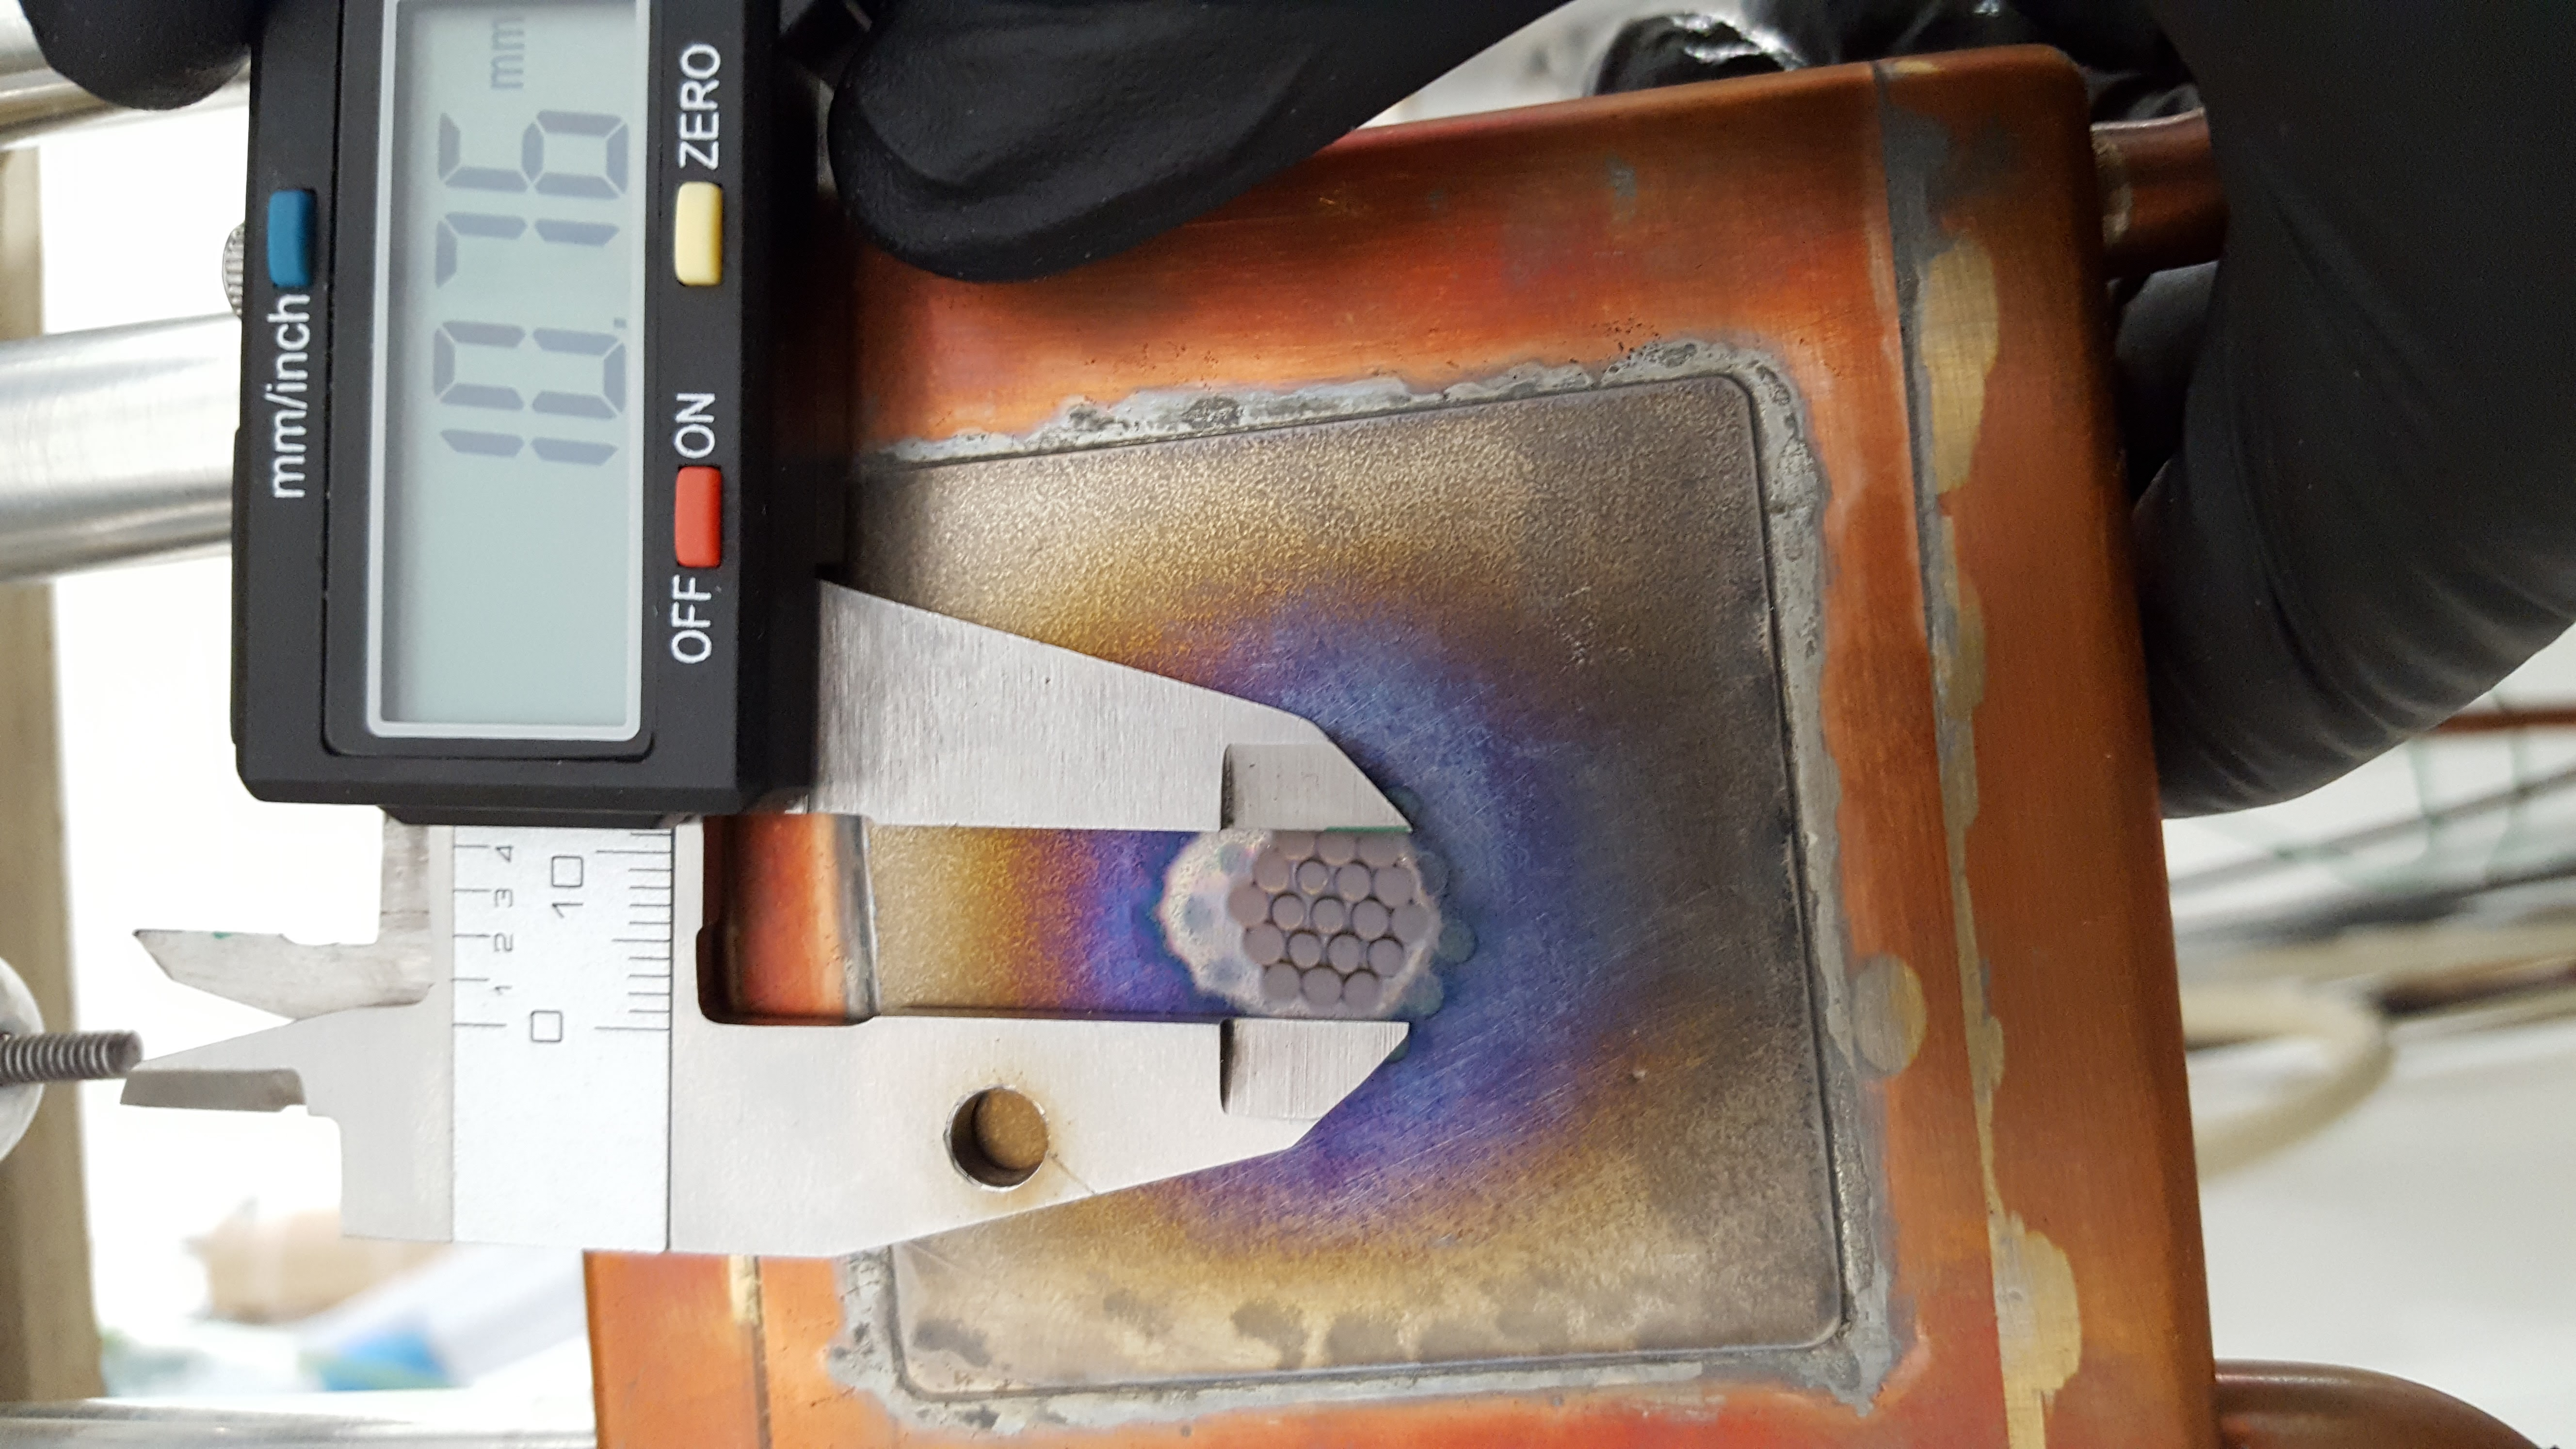
\includegraphics[width=0.9\textwidth]{pics/optimized_notChamfered}
	\caption{Optimized design and resulting beam spot. \DIFaddbeginFL \DIFaddFL{Compared to Figure  \ref{fig:chamfered}, hot spots are almost completely eliminated, and a far more uniform heat pattern is visible.}\DIFaddendFL }
	\label{fig:optimized_notChamfered}
\end{figure}  

The variations in color due to the deuterium beam on the surface of the titanium are an indication of the amount of hydrogen absorbed. \DIFdelbegin \DIFdel{We noticed that after }\DIFdelend \DIFaddbegin \comment{How do you know this? What is the mechanism for the color change?  Explain, and   cite a source.} \DIFadd{Within }\DIFaddend a few minutes of \DIFaddbegin \DIFadd{the end of }\DIFaddend irradiation, the color was black\DIFdelbegin \DIFdel{while after a  long time (hours ) of irradiation, the color becomes light gray.  }\DIFdelend \DIFaddbegin \DIFadd{, but faded to a  light gray after several hours since the end of irradiation.  }\comment{A figure showing the difference in time would be highly valuable here, since you only mention this phenomenon in passing.}
\DIFaddend 

\section{Conclusions and Outlook}

The HFNG is a multi-purpose\DIFaddbegin \DIFadd{, }\DIFaddend versatile neutron generator \DIFdelbegin \DIFdel{that has been well characterized }\DIFdelend \DIFaddbegin \DIFadd{which has been well-characterized }\DIFaddend in terms of flux and energy distribution. Reliable simulation tools \DIFdelbegin \DIFdel{were developed coupled with }\DIFdelend \DIFaddbegin \DIFadd{have been developed and benchmarked through }\DIFaddend experimental validation of the \DIFdelbegin \DIFdel{parameters of interest. Simulations included }\DIFdelend \DIFaddbegin \DIFadd{generator operation. These tools include modeling of the HFNG }\DIFaddend beam optics, heat transfer, neutron flux\DIFdelbegin \DIFdel{and }\DIFdelend \DIFaddbegin \DIFadd{, and neutron }\DIFaddend energy distribution. \DIFaddbegin \DIFadd{Neutron yield and energy distribution has been independently experimentally determined  via indium activation foils. Experimental validation agrees with the simulations described here to within approximately 5}\% \DIFadd{at the sample holder location. 
}\DIFaddend 

Moreover, neutron reflection studies are being investigated in order to increase the neutron fluence in the sample location. \DIFdelbegin \DIFdel{Heavy elements }\DIFdelend \DIFaddbegin \DIFadd{Dense compounds }\DIFaddend such as lead \DIFdelbegin \DIFdel{provide good reflection properties minimizing the }\DIFdelend \DIFaddbegin \DIFadd{or calcium carbonate act as efficient neutron reflectors, minimizing the neutron }\DIFaddend energy loss per collision, which \DIFdelbegin \DIFdel{translates into an overall lower degradation of the }\DIFdelend \DIFaddbegin \DIFadd{prevents significant moderation of the overall }\DIFaddend energy spectrum. 

The heat removal capability of the \DIFaddbegin \DIFadd{HFNG }\DIFaddend target is one of the most important limiting parameters for \DIFdelbegin \DIFdel{neutron flux increase }\DIFdelend \DIFaddbegin \DIFadd{increasing the generator's current neutron flux, }\DIFaddend since hydrogen degases from \DIFdelbegin \DIFdel{titanium if high enough temperatures are achieved}\DIFdelend \DIFaddbegin \DIFadd{the titanium  target without sufficient heat transfer}\DIFaddend . Moreover, the neutron spot size must remain small \DIFaddbegin \comment{Provide an estimate of how large is acceptable} \DIFaddend for the flux to increase linearly with current. \DIFdelbegin \DIFdel{It }\DIFdelend \DIFaddbegin \comment{This is not the best place in the paper to make this claim for the first time.  Bring it up back in the target design sections, and provide a sourec here and there for this claim, since you never brought this up before.} \DIFadd{While it }\DIFaddend is possible to increase the yield by \DIFaddbegin \DIFadd{intentionally }\DIFaddend spreading the beam spot, \DIFdelbegin \DIFdel{but that would not }\DIFdelend \DIFaddbegin \DIFadd{this would }\DIFaddend correspond to a \DIFdelbegin \DIFdel{linear }\DIFdelend \DIFaddbegin \DIFadd{nonlinear }\DIFaddend increase in flux\DIFaddbegin \DIFadd{, which complicates modeling of higher-current designs. 
}

\comment{I think you need to expand the outlook here with more concrete goals for how to continue to imrprove the design, and give commentary on other potential applications for the generator. In particular, point out the potential capabilities of it if we could run DT in a similar design.}

\DIFadd{It is important to note that a high yield neutron generator does not imply  high flux. For instance, commercially available gas-target neutron generators  with DD neutron yields on the order of $10^{11}$}\ \DIFadd{n/s }\comment{DEFINITELY need to cite 1-2 sources for this claim}\DIFadd{. However, the flux at any location around the target is several orders of magnitude lower and impractical for  purposes of geochronology. Moreover, a neutron generator with a solid target but a large beam spot relative to the sample also suffers from the same effect, as the sample is geometrically able to utilize only a fraction of the neutrons produced. In other words, the yield does not scale linearly with  flux as the beam spot increases. }\comment{How does it scale, then?  Inversely?  Please elaborate.} \DIFadd{For an ideal generator, the flux utilization is maximized when operating close to the heat load limit of the target, }\comment{``Therefore'' doesn;t make sense to start this off, as you haven't mentioned heat load limits anywhere else in this paragraph.} \DIFadd{with samples located as close to the neutron production surface as possible, and with  a narrow deuterium beam relative to the size of the target}\DIFaddend .


\DIFaddbegin \comment{I would highly encourage you to read more about teh utilization  factor in our recent (n,p) NIM and elaborate on more of that here, in teh context of the design specifics.}

\DIFaddend \section{Acknowledgments}

We gratefully acknowledge a grant from the University of California Office of the President.

Work supported by NSF Grant No. EAR-0960138, U.S. DOE LBNL Contract No. DE- AC02-05CH11231, and U.S. DOE LLNL Contract No. DE-AC52-07NA27344.

\section*{References}

\DIFdelbegin %DIFDELCMD < \bibliography{mybibfile}
%DIFDELCMD < 	%%%
\DIFdelend \DIFaddbegin \comment{If you submit to NIM, you need to use the elsarticle-num bibliography style.}

\comment{All paper titles listed here have incprrect capitalization - everything is lowercase, aside from teh very first letter.}

\comment{Check your bib file - several entries here appear broken.  [2] is missing my last name and needs to be updated with the volume and page numbers, [5] is missing a last name, [7] is missing a paper title, [8] is missing the author list (\url{https://doi.org/10.13182/NT11-135})}

\comment{When you use \emph{et al.}, it always comes after listing the 3rd author in a list of 3+ authors.  Using the elsarticle-num style should help here, but double check.}

\bibliographystyle{elsarticle-num}

%DIF >  \bibliography{mybibfile}
	\DIFaddend 

\end{document}